% Options for packages loaded elsewhere
\PassOptionsToPackage{unicode}{hyperref}
\PassOptionsToPackage{hyphens}{url}
%
\documentclass[
]{book}
\usepackage{amsmath,amssymb}
\usepackage{lmodern}
\usepackage{ifxetex,ifluatex}
\ifnum 0\ifxetex 1\fi\ifluatex 1\fi=0 % if pdftex
  \usepackage[T1]{fontenc}
  \usepackage[utf8]{inputenc}
  \usepackage{textcomp} % provide euro and other symbols
\else % if luatex or xetex
  \usepackage{unicode-math}
  \defaultfontfeatures{Scale=MatchLowercase}
  \defaultfontfeatures[\rmfamily]{Ligatures=TeX,Scale=1}
\fi
% Use upquote if available, for straight quotes in verbatim environments
\IfFileExists{upquote.sty}{\usepackage{upquote}}{}
\IfFileExists{microtype.sty}{% use microtype if available
  \usepackage[]{microtype}
  \UseMicrotypeSet[protrusion]{basicmath} % disable protrusion for tt fonts
}{}
\makeatletter
\@ifundefined{KOMAClassName}{% if non-KOMA class
  \IfFileExists{parskip.sty}{%
    \usepackage{parskip}
  }{% else
    \setlength{\parindent}{0pt}
    \setlength{\parskip}{6pt plus 2pt minus 1pt}}
}{% if KOMA class
  \KOMAoptions{parskip=half}}
\makeatother
\usepackage{xcolor}
\IfFileExists{xurl.sty}{\usepackage{xurl}}{} % add URL line breaks if available
\IfFileExists{bookmark.sty}{\usepackage{bookmark}}{\usepackage{hyperref}}
\hypersetup{
  pdftitle={ProViz User's Guide},
  hidelinks,
  pdfcreator={LaTeX via pandoc}}
\urlstyle{same} % disable monospaced font for URLs
\usepackage{longtable,booktabs,array}
\usepackage{calc} % for calculating minipage widths
% Correct order of tables after \paragraph or \subparagraph
\usepackage{etoolbox}
\makeatletter
\patchcmd\longtable{\par}{\if@noskipsec\mbox{}\fi\par}{}{}
\makeatother
% Allow footnotes in longtable head/foot
\IfFileExists{footnotehyper.sty}{\usepackage{footnotehyper}}{\usepackage{footnote}}
\makesavenoteenv{longtable}
\usepackage{graphicx}
\makeatletter
\def\maxwidth{\ifdim\Gin@nat@width>\linewidth\linewidth\else\Gin@nat@width\fi}
\def\maxheight{\ifdim\Gin@nat@height>\textheight\textheight\else\Gin@nat@height\fi}
\makeatother
% Scale images if necessary, so that they will not overflow the page
% margins by default, and it is still possible to overwrite the defaults
% using explicit options in \includegraphics[width, height, ...]{}
\setkeys{Gin}{width=\maxwidth,height=\maxheight,keepaspectratio}
% Set default figure placement to htbp
\makeatletter
\def\fps@figure{htbp}
\makeatother
\setlength{\emergencystretch}{3em} % prevent overfull lines
\providecommand{\tightlist}{%
  \setlength{\itemsep}{0pt}\setlength{\parskip}{0pt}}
\setcounter{secnumdepth}{5}
\usepackage{booktabs}
\ifluatex
  \usepackage{selnolig}  % disable illegal ligatures
\fi
\usepackage[]{natbib}
\bibliographystyle{plainnat}

\title{ProViz User's Guide}
\author{}
\date{\vspace{-2.5em}}

\begin{document}
\maketitle

{
\setcounter{tocdepth}{1}
\tableofcontents
}
\hypertarget{proviz}{%
\chapter*{ProViz}\label{proviz}}
\addcontentsline{toc}{chapter}{ProViz}

ProViz is a data visualization and analysis tool developed at SomaLogic. ProViz imports an ADAT file (SomaLogic's data file format) and allows users to perform various exploratory data analytic processes:

\begin{itemize}
\tightlist
\item
  Filter the ADAT to only the samples with desired characteristics
\item
  Merge additional sample data with the data contained in the ADAT
\item
  Create groups of data through aggregating samples or splitting at specific data points
\item
  Create interactive boxplots, CDFs, and scatter plots
\item
  Perform basic statistical tests including correlation, t-test, U-test, KS-tests, ANOVA, and Kruskal\_Wallis.
\end{itemize}

\hypertarget{license}{%
\section*{License}\label{license}}
\addcontentsline{toc}{section}{License}

ProViz is distributed under the MIT License and use of ProViz constitutes acceptance of this license.

MIT License

Copyright © 2021 SomaLogic, Inc.

Permission is hereby granted, free of charge, to any person obtaining a copy of the ProViz software and associated documentation files (the ``Software''), to deal in the Software without restriction, including without limitation the rights to use, copy, modify, merge, publish, distribute, sublicense, and/or sell copies of the Software, and to permit persons to whom the Software is furnished to do so, subject to the following conditions outlined below. Further, ProViz and SomaLogic are trademarks owned by SomaLogic, Inc.~No license is hereby granted to these trademarks other than for purposes of identifying the origin or source of the Software.

The above copyright notice and this permission notice shall be included in all copies or substantial portions of the Software.

THE SOFTWARE IS PROVIDED ``AS IS'', WITHOUT WARRANTY OF ANY KIND, EXPRESS OR IMPLIED, INCLUDING BUT NOT LIMITED TO THE WARRANTIES OF MERCHANTABILITY, FITNESS FOR A PARTICULAR PURPOSE AND NONINFRINGEMENT. IN NO EVENT SHALL THE AUTHORS OR COPYRIGHT HOLDER(S) BE LIABLE FOR ANY CLAIM, DAMAGES, WHETHER DIRECT OR INDIRECT, OR OTHER LIABILITY, WHETHER IN AN ACTION OF CONTRACT, TORT OR OTHERWISE, ARISING FROM, OUT OF OR IN CONNECTION WITH THE SOFTWARE OR THE USE OR OTHER DEALINGS IN THE SOFTWARE.

\hypertarget{installation-and-prerequisites}{%
\chapter{Installation and Prerequisites}\label{installation-and-prerequisites}}

\hypertarget{installation}{%
\section{Installation}\label{installation}}

\hypertarget{github}{%
\subsection{GitHub}\label{github}}

ProViz is a Shiny application written in R. The source code is available on GitHub in SomaLogic's \href{https://github.com/SomaLogic/ProViz}{ProViz repository}.

To use ProViz, it is recommended to install RStudio, clone the ProViz repository, and run it using the RStudio IDE. See \href{https://shiny.rstudio.com/}{RStudio's Shiny page} for details of using RStudio to run a Shiny application. \href{https://rstudio.com/products/shiny/shiny-server/}{RStudio's Shiny Server} can also be used to run ProViz from a server, providing access through a managed web portal.

Some additional packages are required for ProViz. Following is a list of the required packages and the versions used during ProViz development and testing. All of the following packages are available through \href{https://cran.r-project.org/}{The Comprehensive R Network - CRAN}.

\begin{itemize}
\tightlist
\item
  shiny (1.6.0)
\item
  shinydashboard (0.7.1)
\item
  shinyWidgets (0.6.0)
\item
  DT (0.17)
\item
  dplyr (1.0.5)
\item
  ggbeeswarm (0.6.0)
\item
  ggplot2 (3.3.3)
\item
  magrittr (2.0.1)
\item
  plotly (4.9.3)
\item
  readr (1.4.0)
\item
  tidyr (1.0.2)
\end{itemize}

Additionally, ProViz uses the SomaDataIO v5.0.0 package available from \href{https://github.com/SomaLogic/SomaDataIO}{SomaLogic's SomaDataIO GitHub repository}. Note that SomaDataIO requires the BioBase package from \href{https://bioconductor.org/}{Bioconductor}, which requires a slightly different installation procedure:

\begin{verbatim}
if (!requireNamespace("BiocManager", quietly = TRUE)) {
  install.packages("BiocManager")
}
BiocManager::install("Biobase")
\end{verbatim}

Installing dependencies can be accomplished using the \texttt{remotes} package and the following series of R commands.

\begin{verbatim}
# install the remotes package 
install.packages('remotes')

# install the individual dependencies
remotes::install_version('DT', version = '0.17', 
                         repos = 'http://cran.us.r-project.org')
remotes::install_version('dplyr', version = '1.0.5',
                         repos = 'http://cran.us.r-project.org')
remotes::install_version('ggbeeswarm', version = '0.6.0',
                         repos = 'http://cran.us.r-project.org')
remotes::install_version('ggplot2', version = '3.3.3',
                         repos = 'http://cran.us.r-project.org')
remotes::install_version('magrittr', version = '2.0.1',
                         repos = 'http://cran.us.r-project.org')
remotes::install_version('plotly', version = '4.9.3',
                         repos = 'http://cran.us.r-project.org')
remotes::install_version('readr', version = '1.4.0',
                         repos = 'http://cran.us.r-project.org')
remotes::install_version('shiny', version = '1.6.0',
                         repos = 'http://cran.us.r-project.org')
remotes::install_version('shinydashboard', version = '0.7.1',
                         repos = 'http://cran.us.r-project.org')
remotes::install_version('shinyWidgets', version = '0.6.0',
                         repos = 'http://cran.us.r-project.org')
remotes::install_version('tidyr', version = '1.0.2',
                         repos = 'http://cran.us.r-project.org')
remotes::install_version('usethis', version = '1.6.0',
                         repos = 'http://cran.us.r-project.org')
remotes::install_github('Somalogic/SomaDataIO@v5.0.0')
\end{verbatim}

\hypertarget{dockerhub}{%
\subsection{DockerHub}\label{dockerhub}}

ProViz can also be run using Docker or Docker Desktop using the image available through \href{https://hub.docker.com/r/somalogic/proviz}{SomaLogic's Dockerhub account}. For more information on installing and running Docker Desktop, refer to the \href{https://www.docker.com/products/docker-desktop}{Docker Desktop home page}.

Once Docker Desktop is installed, the ProViz image can be pulled from dockerhub by executing \texttt{docker\ pull\ somalogic/proviz} from a terminal window on Mac or Linux, or from a command prompt on Windows. Once the image has been successfully pulled, the image name will be displayed in the Docker Desktop's Dashboard application.

\begin{figure}
\centering
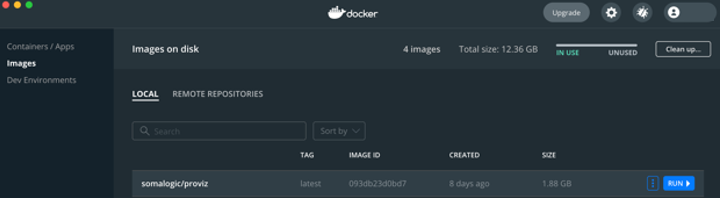
\includegraphics{images/Dashboard.png}
\caption{Docker Dashboard showing the ProViz image available.}
\end{figure}

The image can be started by clicking run. A dialog box will be presented in which a local port number needs to be set (Local Port) in order for a web browser to communicate with the running container. Any available port can be used, and the default 3838 is most likely a good option. (You may initially see a smaller dialog box with the port setting hidden. Clicking on the triangle at the right will expand the dialog to show all options.)

\begin{figure}
\centering
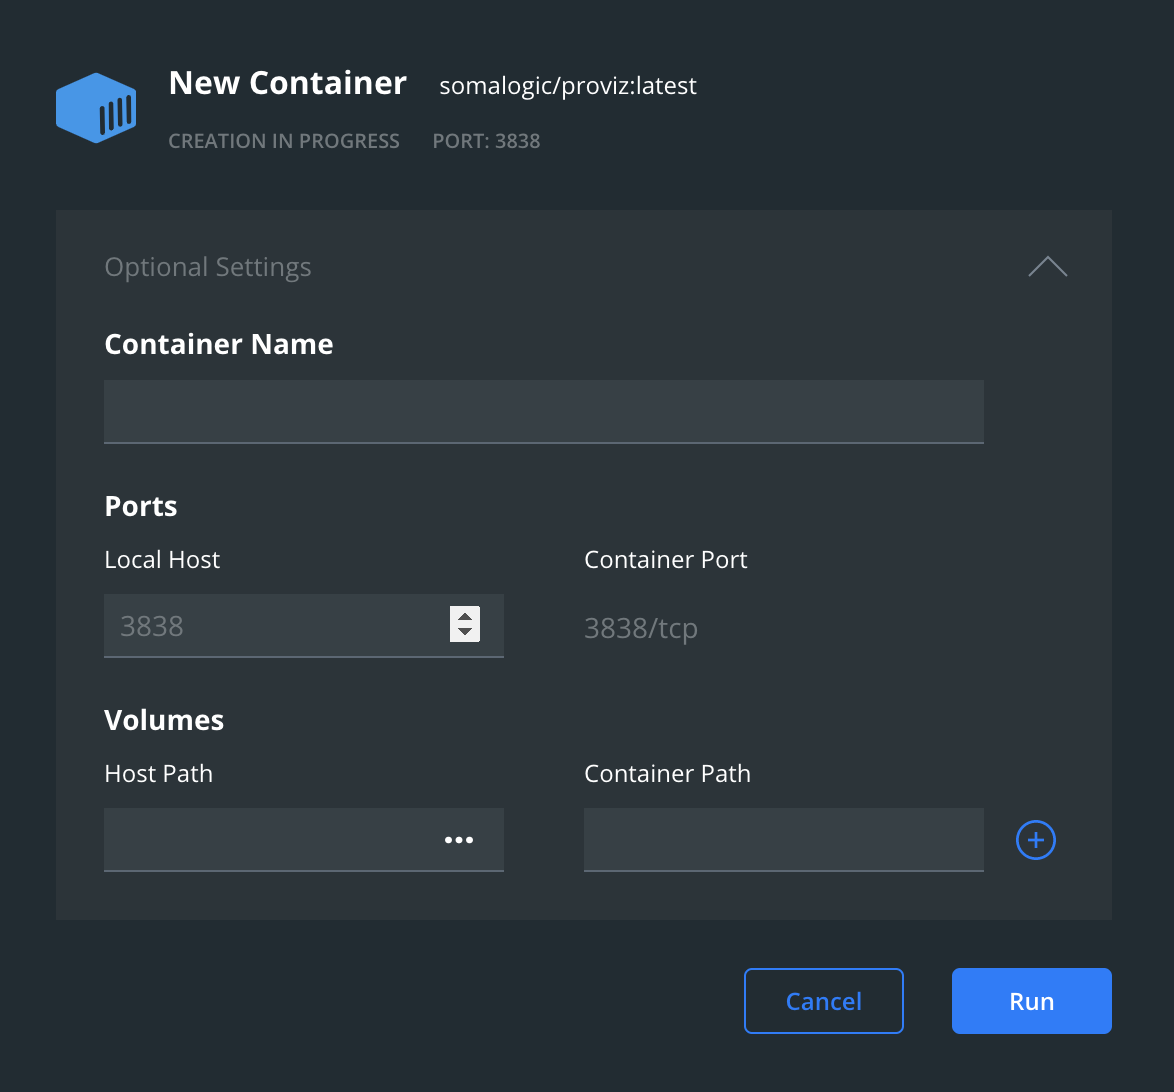
\includegraphics{images/Dashboard_port.png}
\caption{Setting the Local Port to 3838.}
\end{figure}

Once the Local Port is set, click Run. in the Dashboard, you will now see that the image is running. Clicking on Open in Browser will connect your web browser to the container through the Local Port set in the last step.

\begin{figure}
\centering
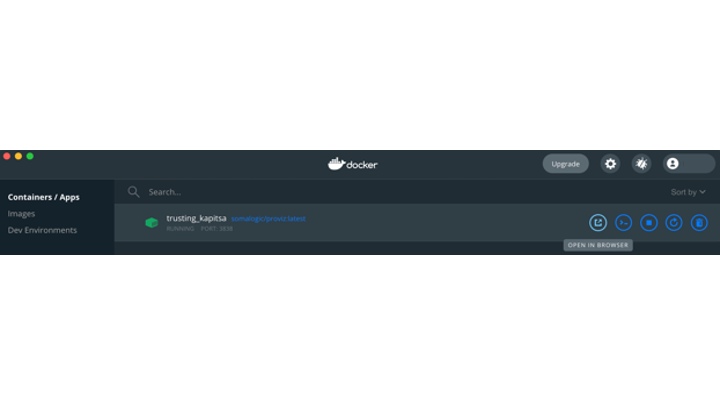
\includegraphics{images/Dashboard_runningimage.png}
\caption{Docker Dashboard showing that the container is running.}
\end{figure}

When your browser opens, you should see the Shiny Server welcome page.

\begin{figure}
\centering
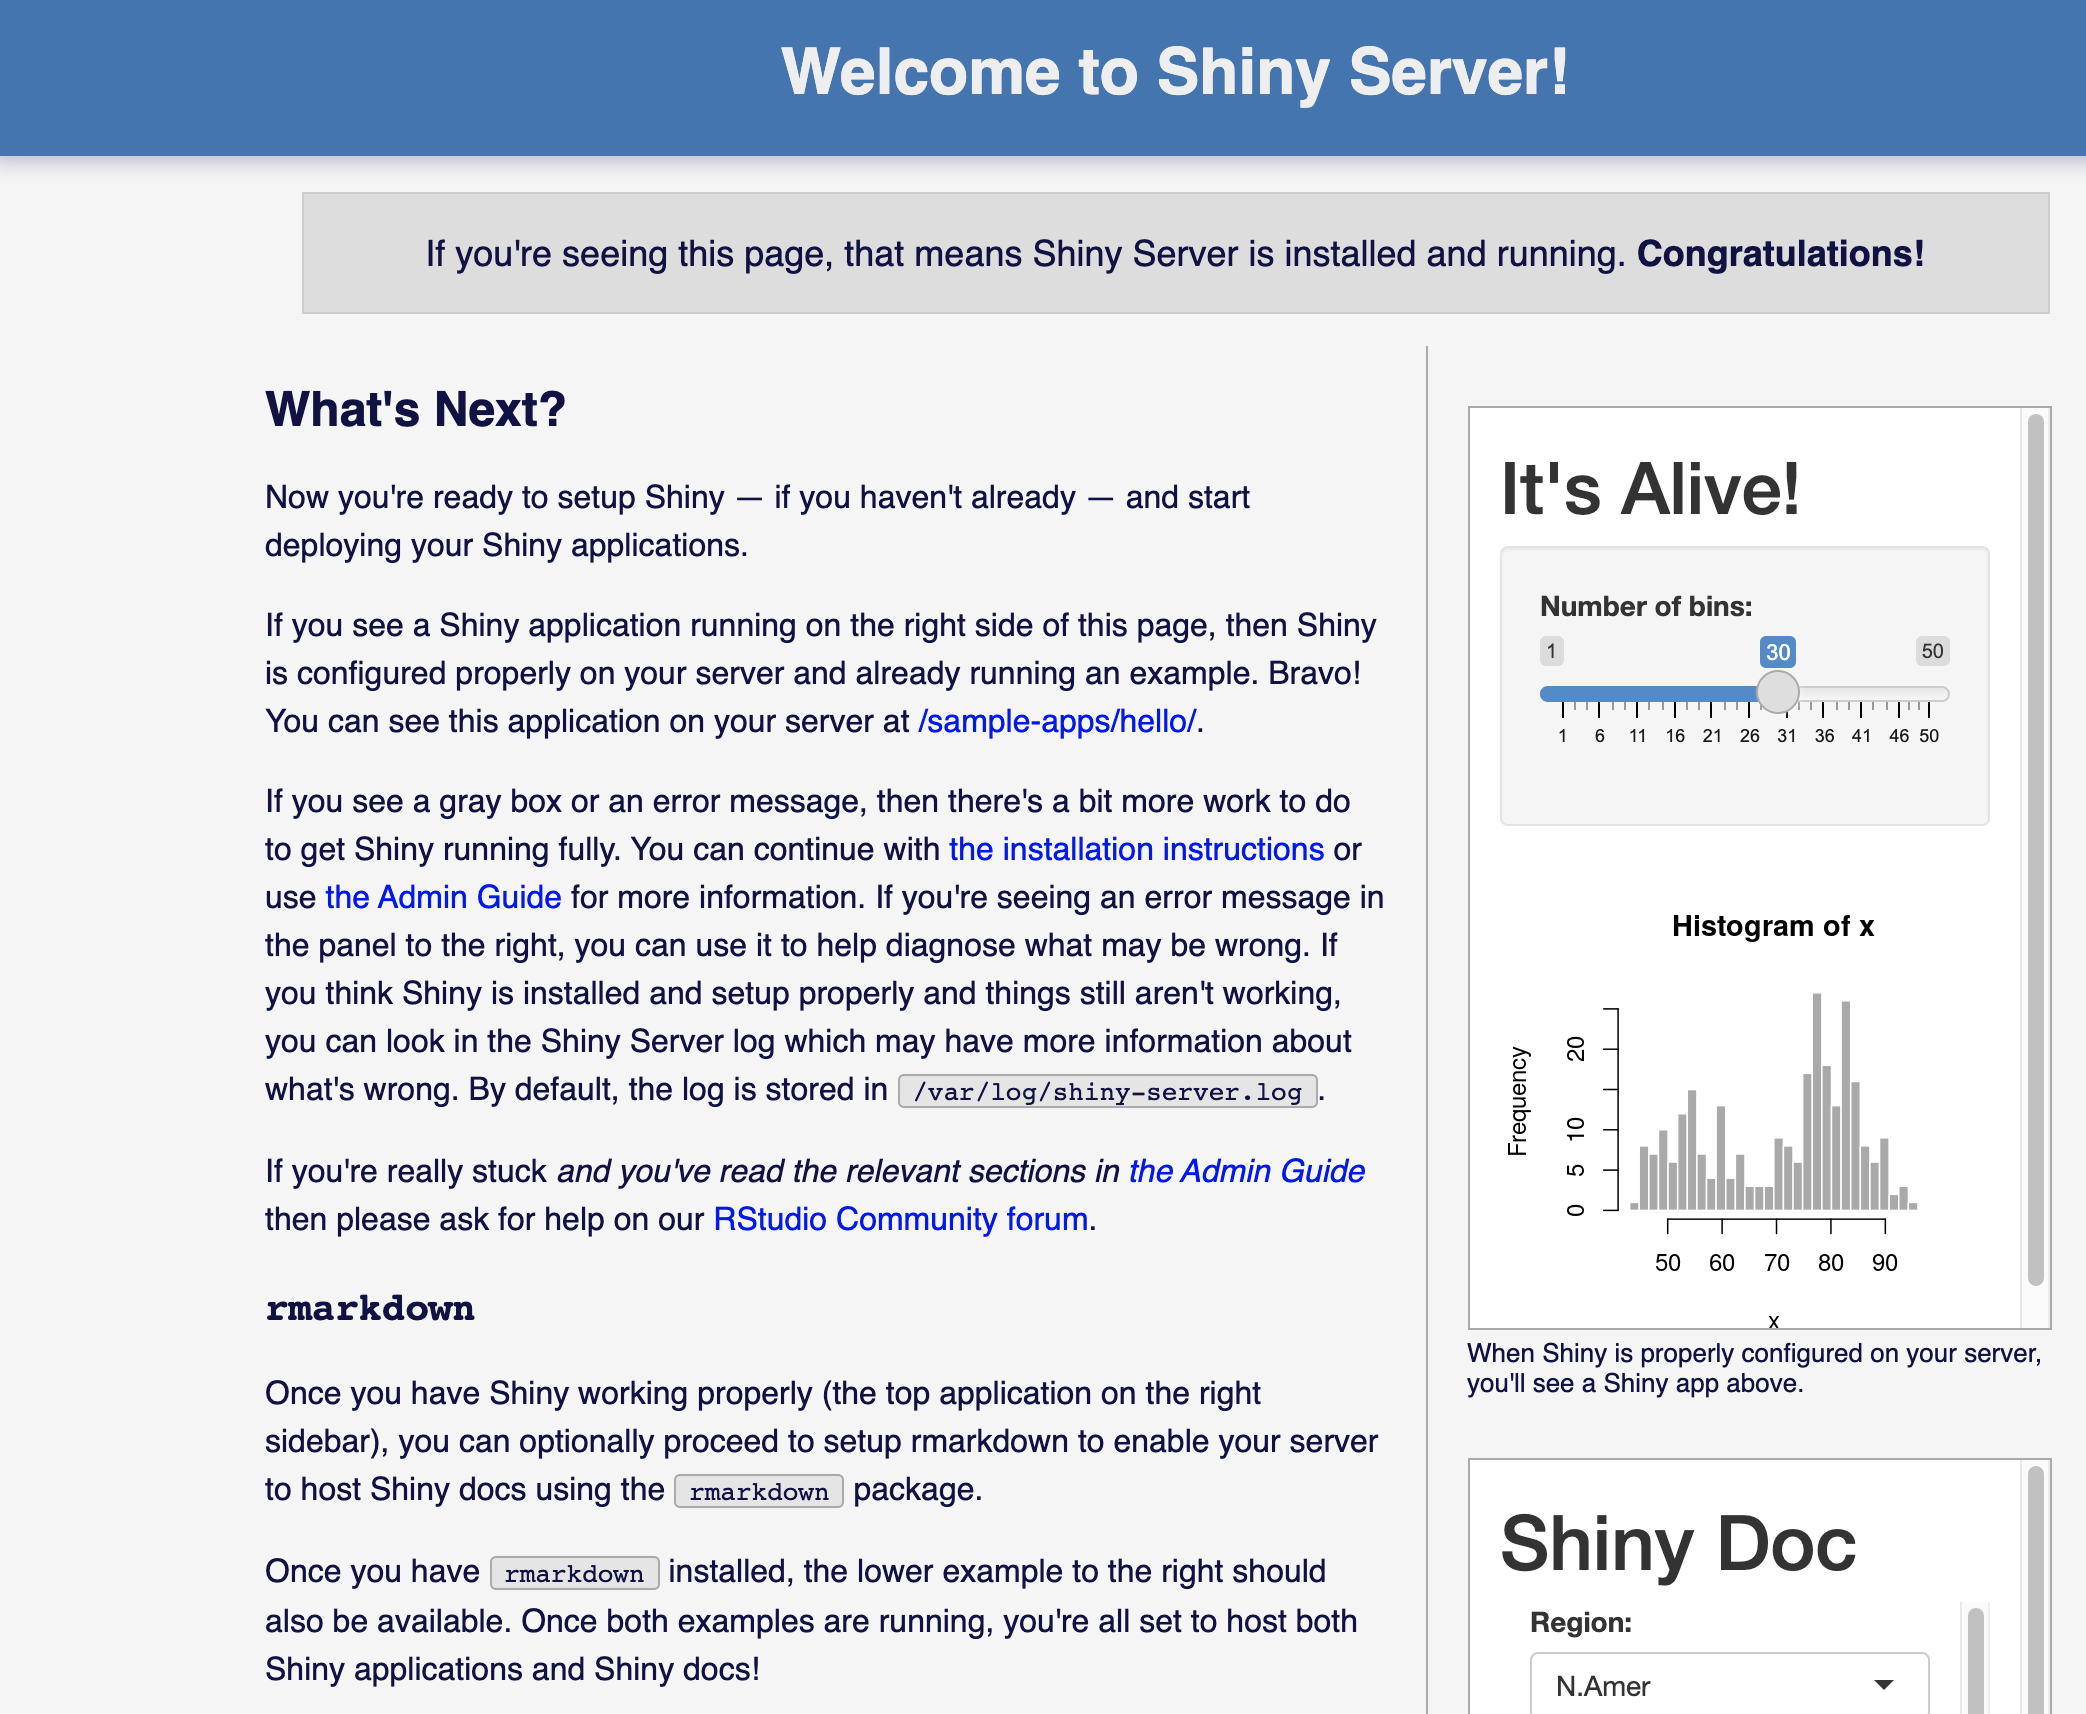
\includegraphics{images/ShinyWelcome.png}
\caption{Shiny Server welcome page.}
\end{figure}

To access Proviz, just add ``/ProViz'' to the end of the address in the browser.

\begin{figure}
\centering

\includegraphics{images/ProVizURL.png}
\caption{The full ProViz URL.}
\end{figure}

\hypertarget{example-data}{%
\section{Example Data}\label{example-data}}

The example data used in this tutorial can be found at SomaLogic's \href{https://github.com/SomaLogic/SomaLogic-Data}{SomaLogic-Data GitHub repository} where you can find a description of the file and the ADAT file format. The \texttt{example\_data.adat} file consists of 192 samples (including clinical samples and controls) and is representative of a typical ADAT file SomaLogic customer's receive.

\hypertarget{proviz-navigation}{%
\section{ProViz Navigation}\label{proviz-navigation}}

\begin{figure}
\centering

\includegraphics{images/ProViz_main.png}
\caption{The main ProViz panel.}
\end{figure}

In ProViz, you can navigate to different panels using the navigation pane on the left by clicking on the name of the panel. Each chapter in this tutorial gives a brief tutorial on how to use the options in the corresponding panel.

Users can select how the SOMAmer-associated data will be listed in selection boxes across all ProViz panels by selecting an option under \textbf{Label SOMAmers by}: \emph{SOMAmer ID}, \emph{Protein Name}, or \emph{Gene Symbol}. The latter two options are most likely more familiar to most users than SOMAmer IDs. Label types can be changed at any point when using ProViz.

\hypertarget{load-and-filter-adat}{%
\chapter{Load and Filter ADAT}\label{load-and-filter-adat}}

\hypertarget{the-load-and-filter-adat-panel}{%
\section{The Load and Filter ADAT Panel}\label{the-load-and-filter-adat-panel}}

\begin{figure}
\centering
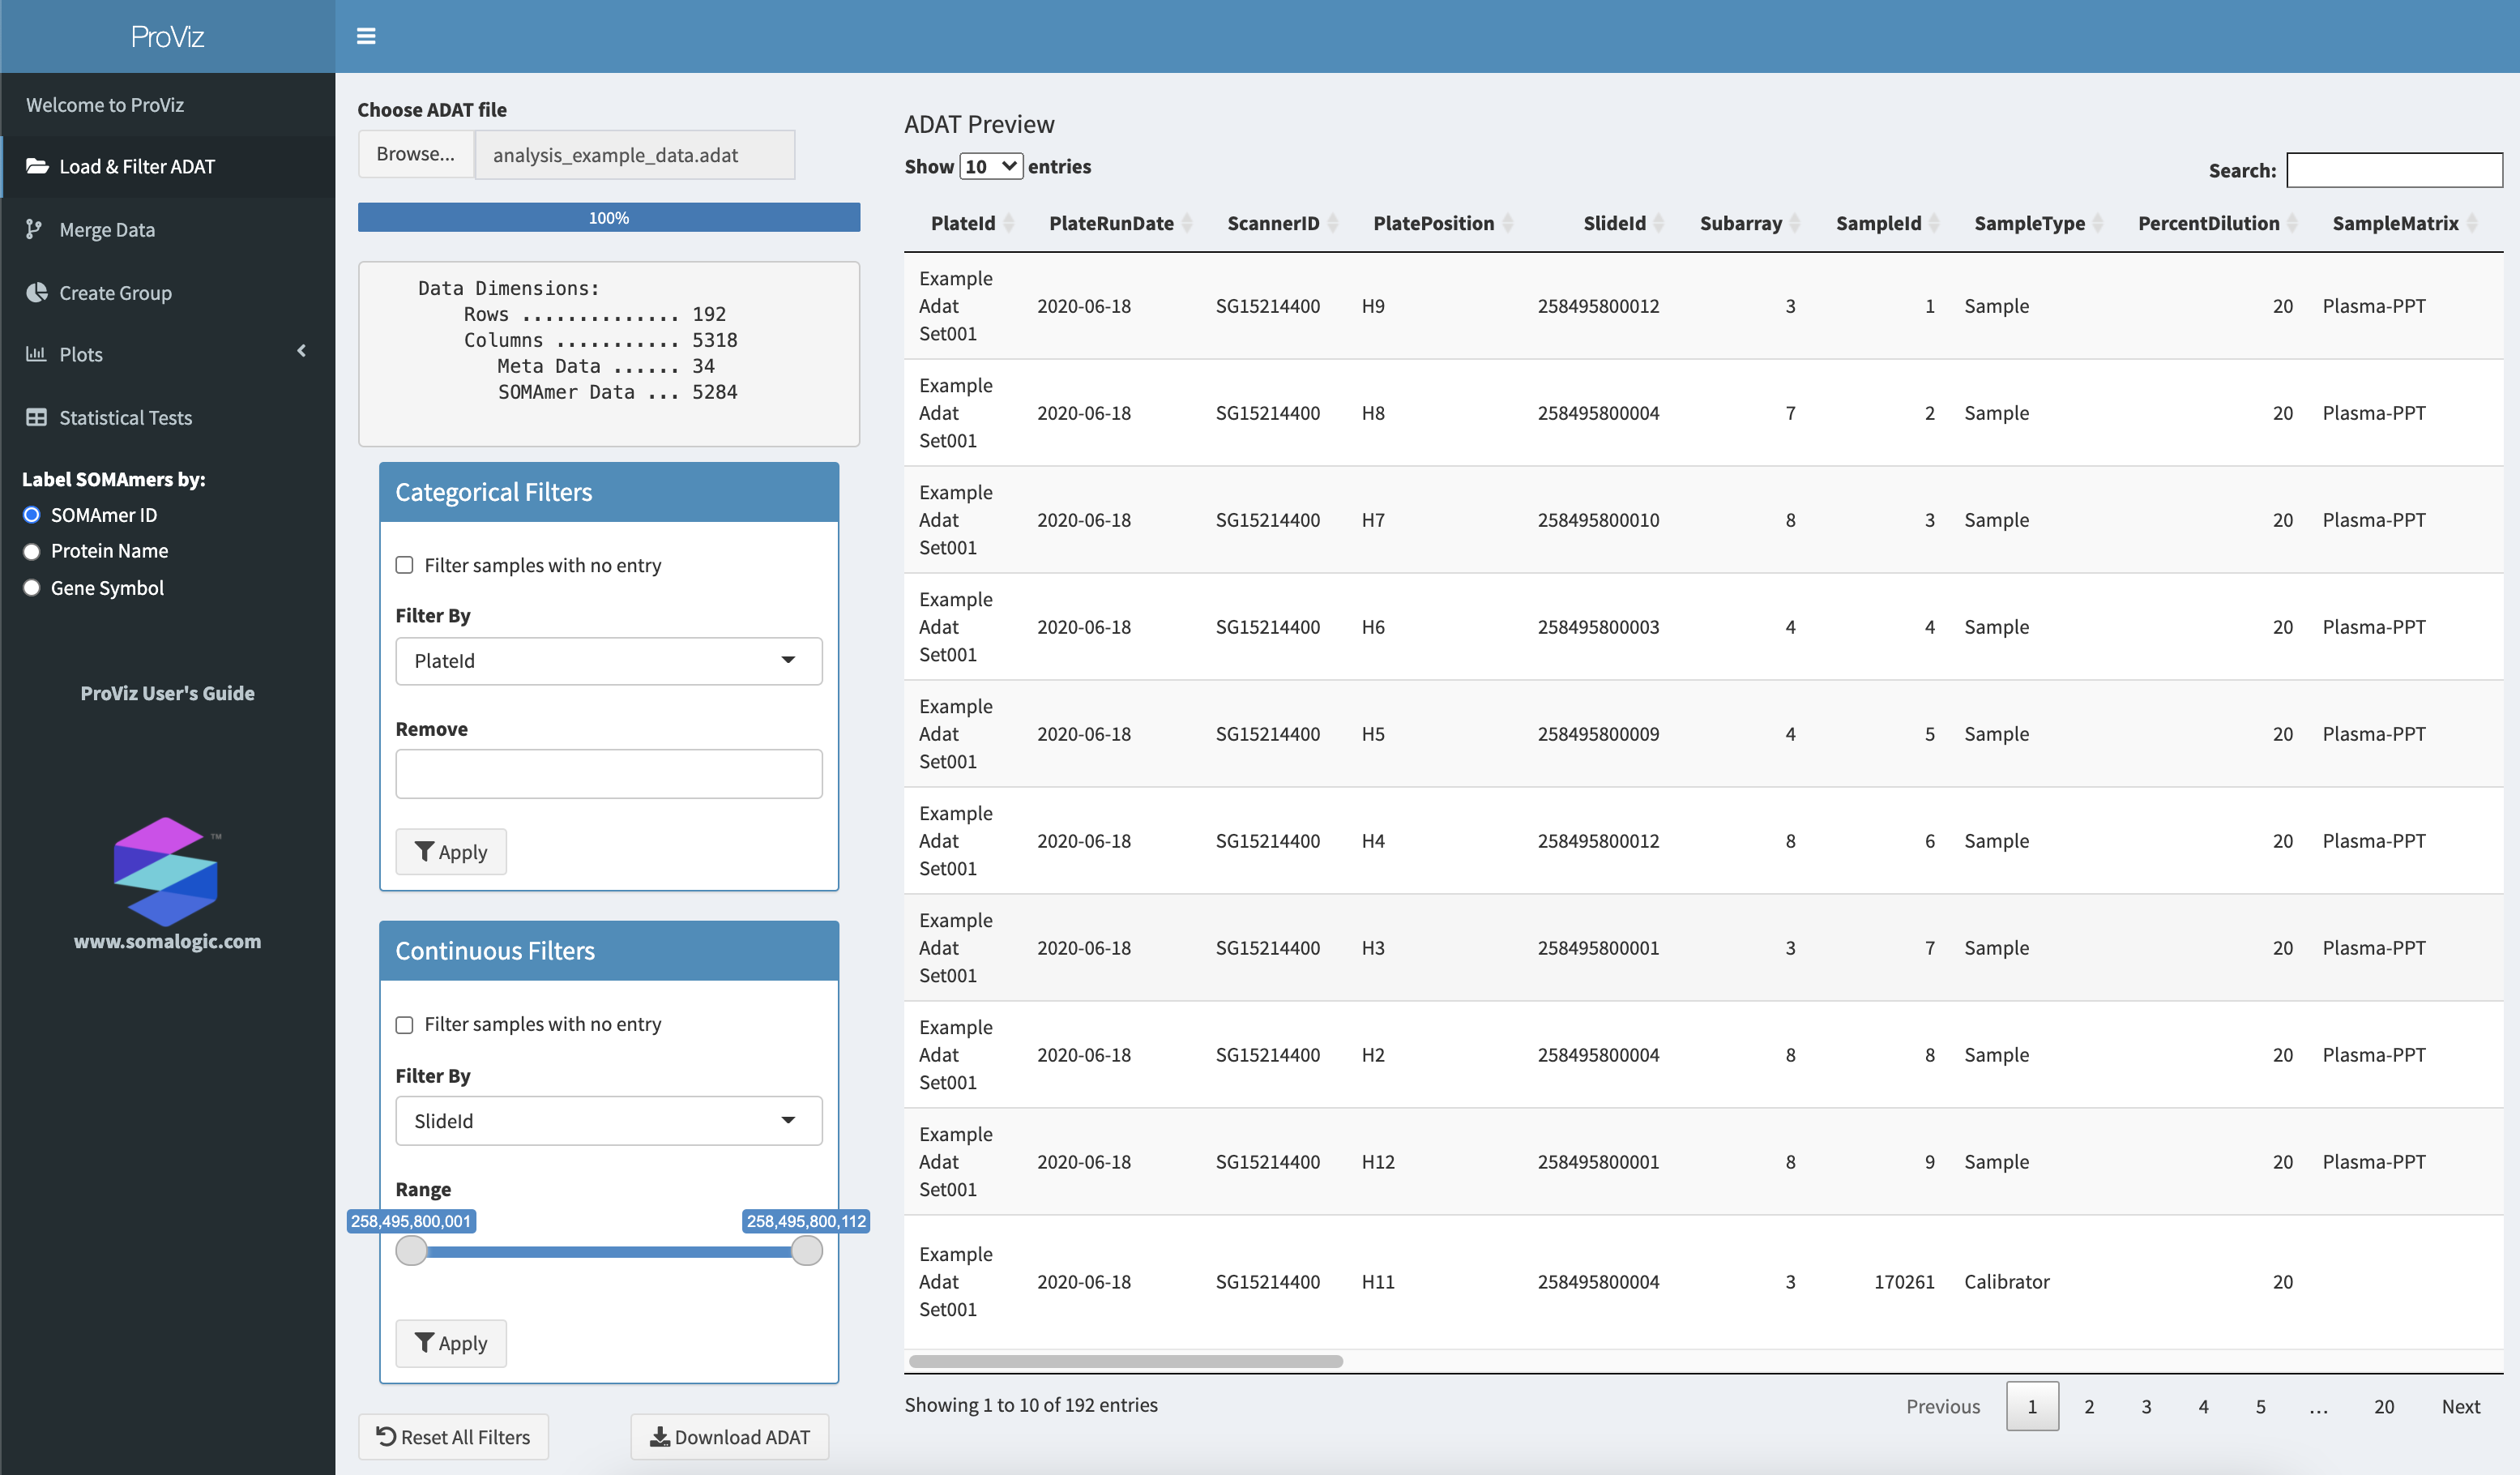
\includegraphics{images/LoadAndFilter.png}
\caption{The ProViz Load and Filter ADAT panel after opening the \texttt{example\_data.adat} file.}
\end{figure}

\hypertarget{load-an-adat-file}{%
\section{Load an ADAT file}\label{load-an-adat-file}}

To open an ADAT file, click on the \textbf{Browse\ldots{}} button and locate an ADAT file. Once selected, the ADAT file will be opened and processed, and a preview of the content will be shown in the table at the right. ADAT files may have over 7,000 columns of SomaScan Assay data for every row in the file, so large files may take a few moments to load.

After the ADAT file is loaded, details of the file content are displayed. Here we see that there are 192 total rows (corresponding to individual samples), and 5,318 data columns. Of those data columns, 5,284 are SOMAmer data columns and 34 are Meta Data columns. These Meta Data columns contain assay-related data such as the Plate ID, Scanner ID, normalization data, and any sample-specific data that was submitted to SomaLogic with the samples. For the \texttt{example\_data.adat} file, Sex and Age are included as well as various assay-related content.

The ADAT Preview table can be scroleld as well as searched for specific content (\textbf{Search:} box in upper-right). SomaScan Assay data are not displayed in the preview table.

\hypertarget{filter-adat-contents}{%
\section{Filter ADAT contents}\label{filter-adat-contents}}

Samples present in the ADAT file can be filtered based on Meta Data or SomaScan Assay data. When the ADAT file is processed, data columns are divided into Categorical (non-numeric) or Continuous (numeric) categories.

All filtering operations are cumulative.

\hypertarget{categorical-filters}{%
\subsection{Categorical Filters}\label{categorical-filters}}

\begin{figure}
\centering
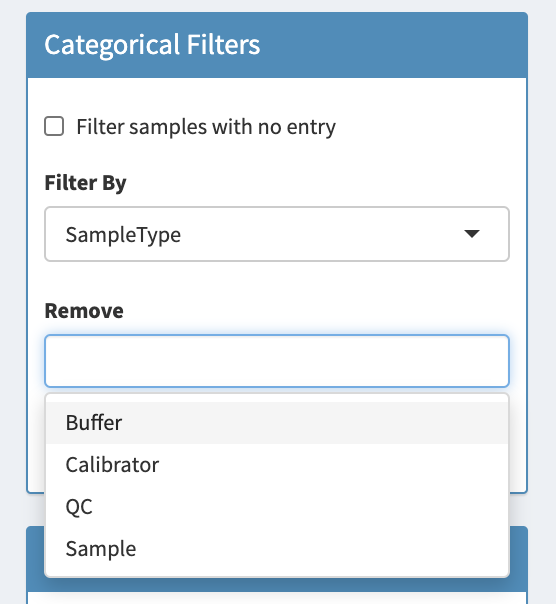
\includegraphics{images/CategoricalFilters.png}
\caption{The categorical filters box.}
\end{figure}

Samples can be filtered from the ADAT based on categorical data using the Categorical Filters box. The column name can be selected from the \textbf{Filter By} selection box, which populates the \textbf{Remove} selection box with the unique categorical values in the ADAT file. Data values can be selected by clicking on one or more values in the \textbf{Remove} selection box. Once all selections are made, clicking the \textbf{Apply} button will remove those samples from the data, and the Data Dimensions box will be updated with new information.

In this example, the \emph{SampleType} column is selected and the unique entries for this column are shown: Buffer, Calibrator, QC, and Sample. By clicking on Buffer, Calibrator, and QC, to select them, the assay control samples can be removed from the data file.

Checking the \textbf{Filter samples with no entry} box will remove all samples lacking a value for the selected column.

\hypertarget{continuous-filters}{%
\subsection{Continuous Filters}\label{continuous-filters}}

\begin{figure}
\centering
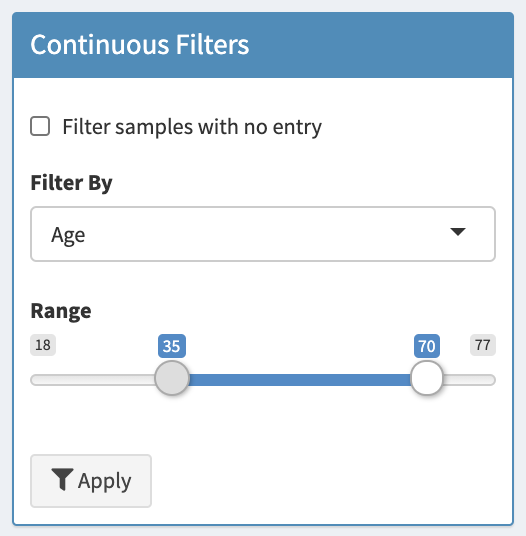
\includegraphics{images/ContinousFilters.png}
\caption{The continuous filters box.}
\end{figure}

Samples can be filtered from the ADAT based on continuous data using the Continuous Filters box. The column name can be selected from the \textbf{Filter By} which will update the \textbf{Range} slider with the minimum and maximum values for that data column. By moving the minimum and maximum sliders, a desired range of the selected variable can be chosen and all samples with values outside that range will be removed.

In this example, the \emph{Age} column is seleted and the sliders adjusted to keep only those samples with Age from 35 to 70.

Checking the \textbf{Filter samples with no entry} box will remove all samples lacking a value for the selected column.

\hypertarget{reset-filters}{%
\subsection{Reset Filters}\label{reset-filters}}

The original ADAT contents are always preserved and can be retrieved by clicking the \textbf{Reset All Filters} button.

\hypertarget{download-adat}{%
\subsection{Download ADAT}\label{download-adat}}

Once filtering has been performed, a version of the ADAT can be downloaded by clicking the \textbf{Download ADAT} button. As this new ADAT file may be significantly modified relative to the original, ensure that a new, unique, descriptive file name is specified so that the original ADAT is not overwritten. Keeping good notes regarding the filtering operations is essential to recall how the ADAT was modified when it is returned to at a later date.

\hypertarget{merge-data}{%
\chapter{Merge Data}\label{merge-data}}

Data stored in external files can be merged with the proteomic data in an ADAT file using the Merge Data panel.

\begin{figure}
\centering
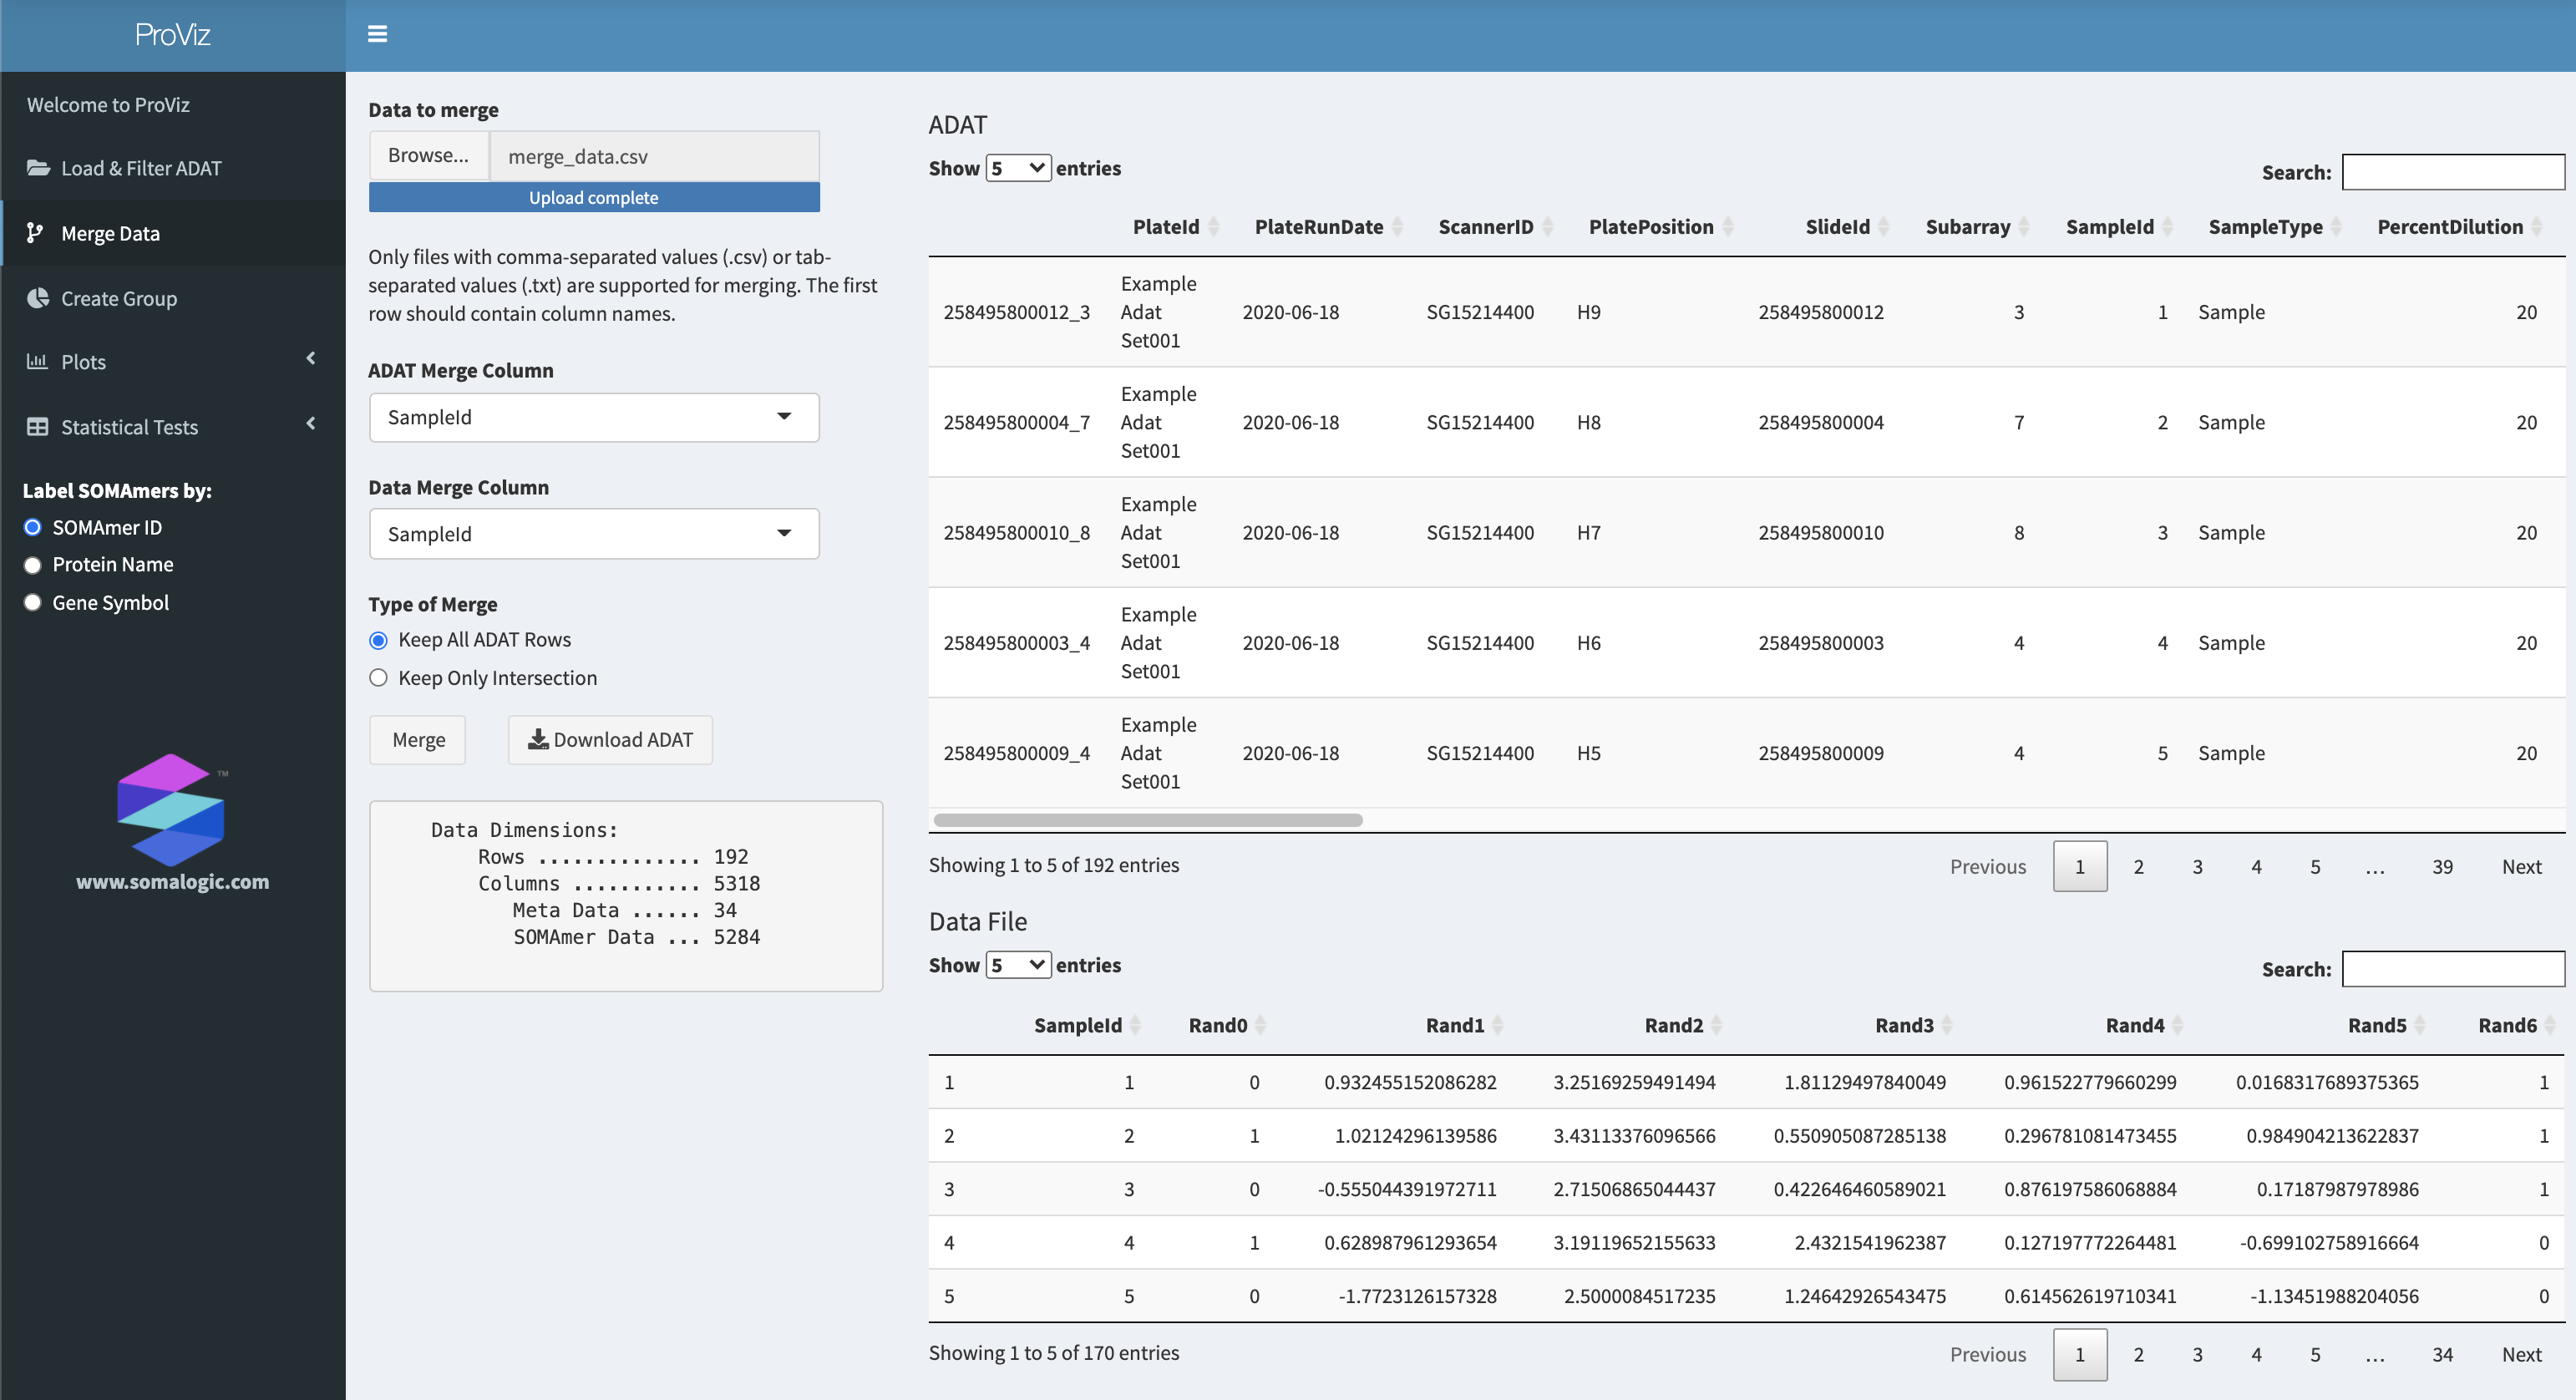
\includegraphics{images/MergeData.png}
\caption{The Merge Data panel}
\end{figure}

\hypertarget{selecting-a-data-file-to-merge}{%
\section{Selecting a Data File to Merge}\label{selecting-a-data-file-to-merge}}

External data must be stored in a comma-delimited or a tab-delimited file, and the first row should contain column names. The file containing the data can be uploaded to ProViz by selecting the Browse button and navigating to the file. Once uploaded, a preview of the data file will be displayed below the ADAT Preview.

\hypertarget{selecting-columns-in-the-adat-and-the-data-file}{%
\section{Selecting Columns in the ADAT and the Data File}\label{selecting-columns-in-the-adat-and-the-data-file}}

In order to merge external data with the data in the ADAT file, each file should have one column that provides a way to match rows between the two files. Ideally, the columns should have all unique values and should match one-to-one between the ADAT file and the external data file. The target column in the ADAT can be selected with the \textbf{ADAT Merge Column} selection box, and the column in the external file can be selected with the \textbf{Data Merge Column} selection box. The columns do not need to have the same name.

In this example, each file has a column titled SampleId. All entries in this column in the external file are unique and correspond to the clinical samples' SampleId values in the ADAT.

\hypertarget{specifying-the-type-of-merge}{%
\section{Specifying the Type of Merge}\label{specifying-the-type-of-merge}}

The ADAT file typically contains control samples for which external data is not likely available, or the external data file may not have data for all clinical samples. Choosing \emph{Keep All ADAT Rows} under \textbf{Type of Merge} will retain all rows in the ADAT file and include \emph{NA} for those rows not found in the external file. Alternatively, only those rows found in both files can be retained by selecting \emph{Keep Only Intersection}.

\hypertarget{merge}{%
\section{Merge}\label{merge}}

Once all selections are made, initiate the merge by pressing the \textbf{Merge} button. If an error occurs, a message will be displayed in the message box at the bottom of the panel, otherwise, the message box will contain updated data dimension information. The message box will provide the exact error message from the underlying R code, and may not be easily interpreted. Typically, if an error occurs, it is due to selecting columns in either the ADAT or the external file that are not campatible.

\hypertarget{download-adat-1}{%
\section{Download Adat}\label{download-adat-1}}

Once merging has been performed, a version of the ADAT can be downloaded by clicking the \textbf{Download ADAT} button. As this new ADAT file may be significantly modified relative to the original, ensure that a new, unique, descriptive file name is specified so that the original ADAT is not overwritten. Keeping good notes regarding the filtering operations is essential to recall how the ADAT was modified when it is returned to at a later date.

\hypertarget{create-group}{%
\chapter{Create Group}\label{create-group}}

New groups can be created from existing data. Samples labeled with categorical data can be combined to create only 2 groups, or continuous values can be split to create 2 groups.

\begin{figure}
\centering
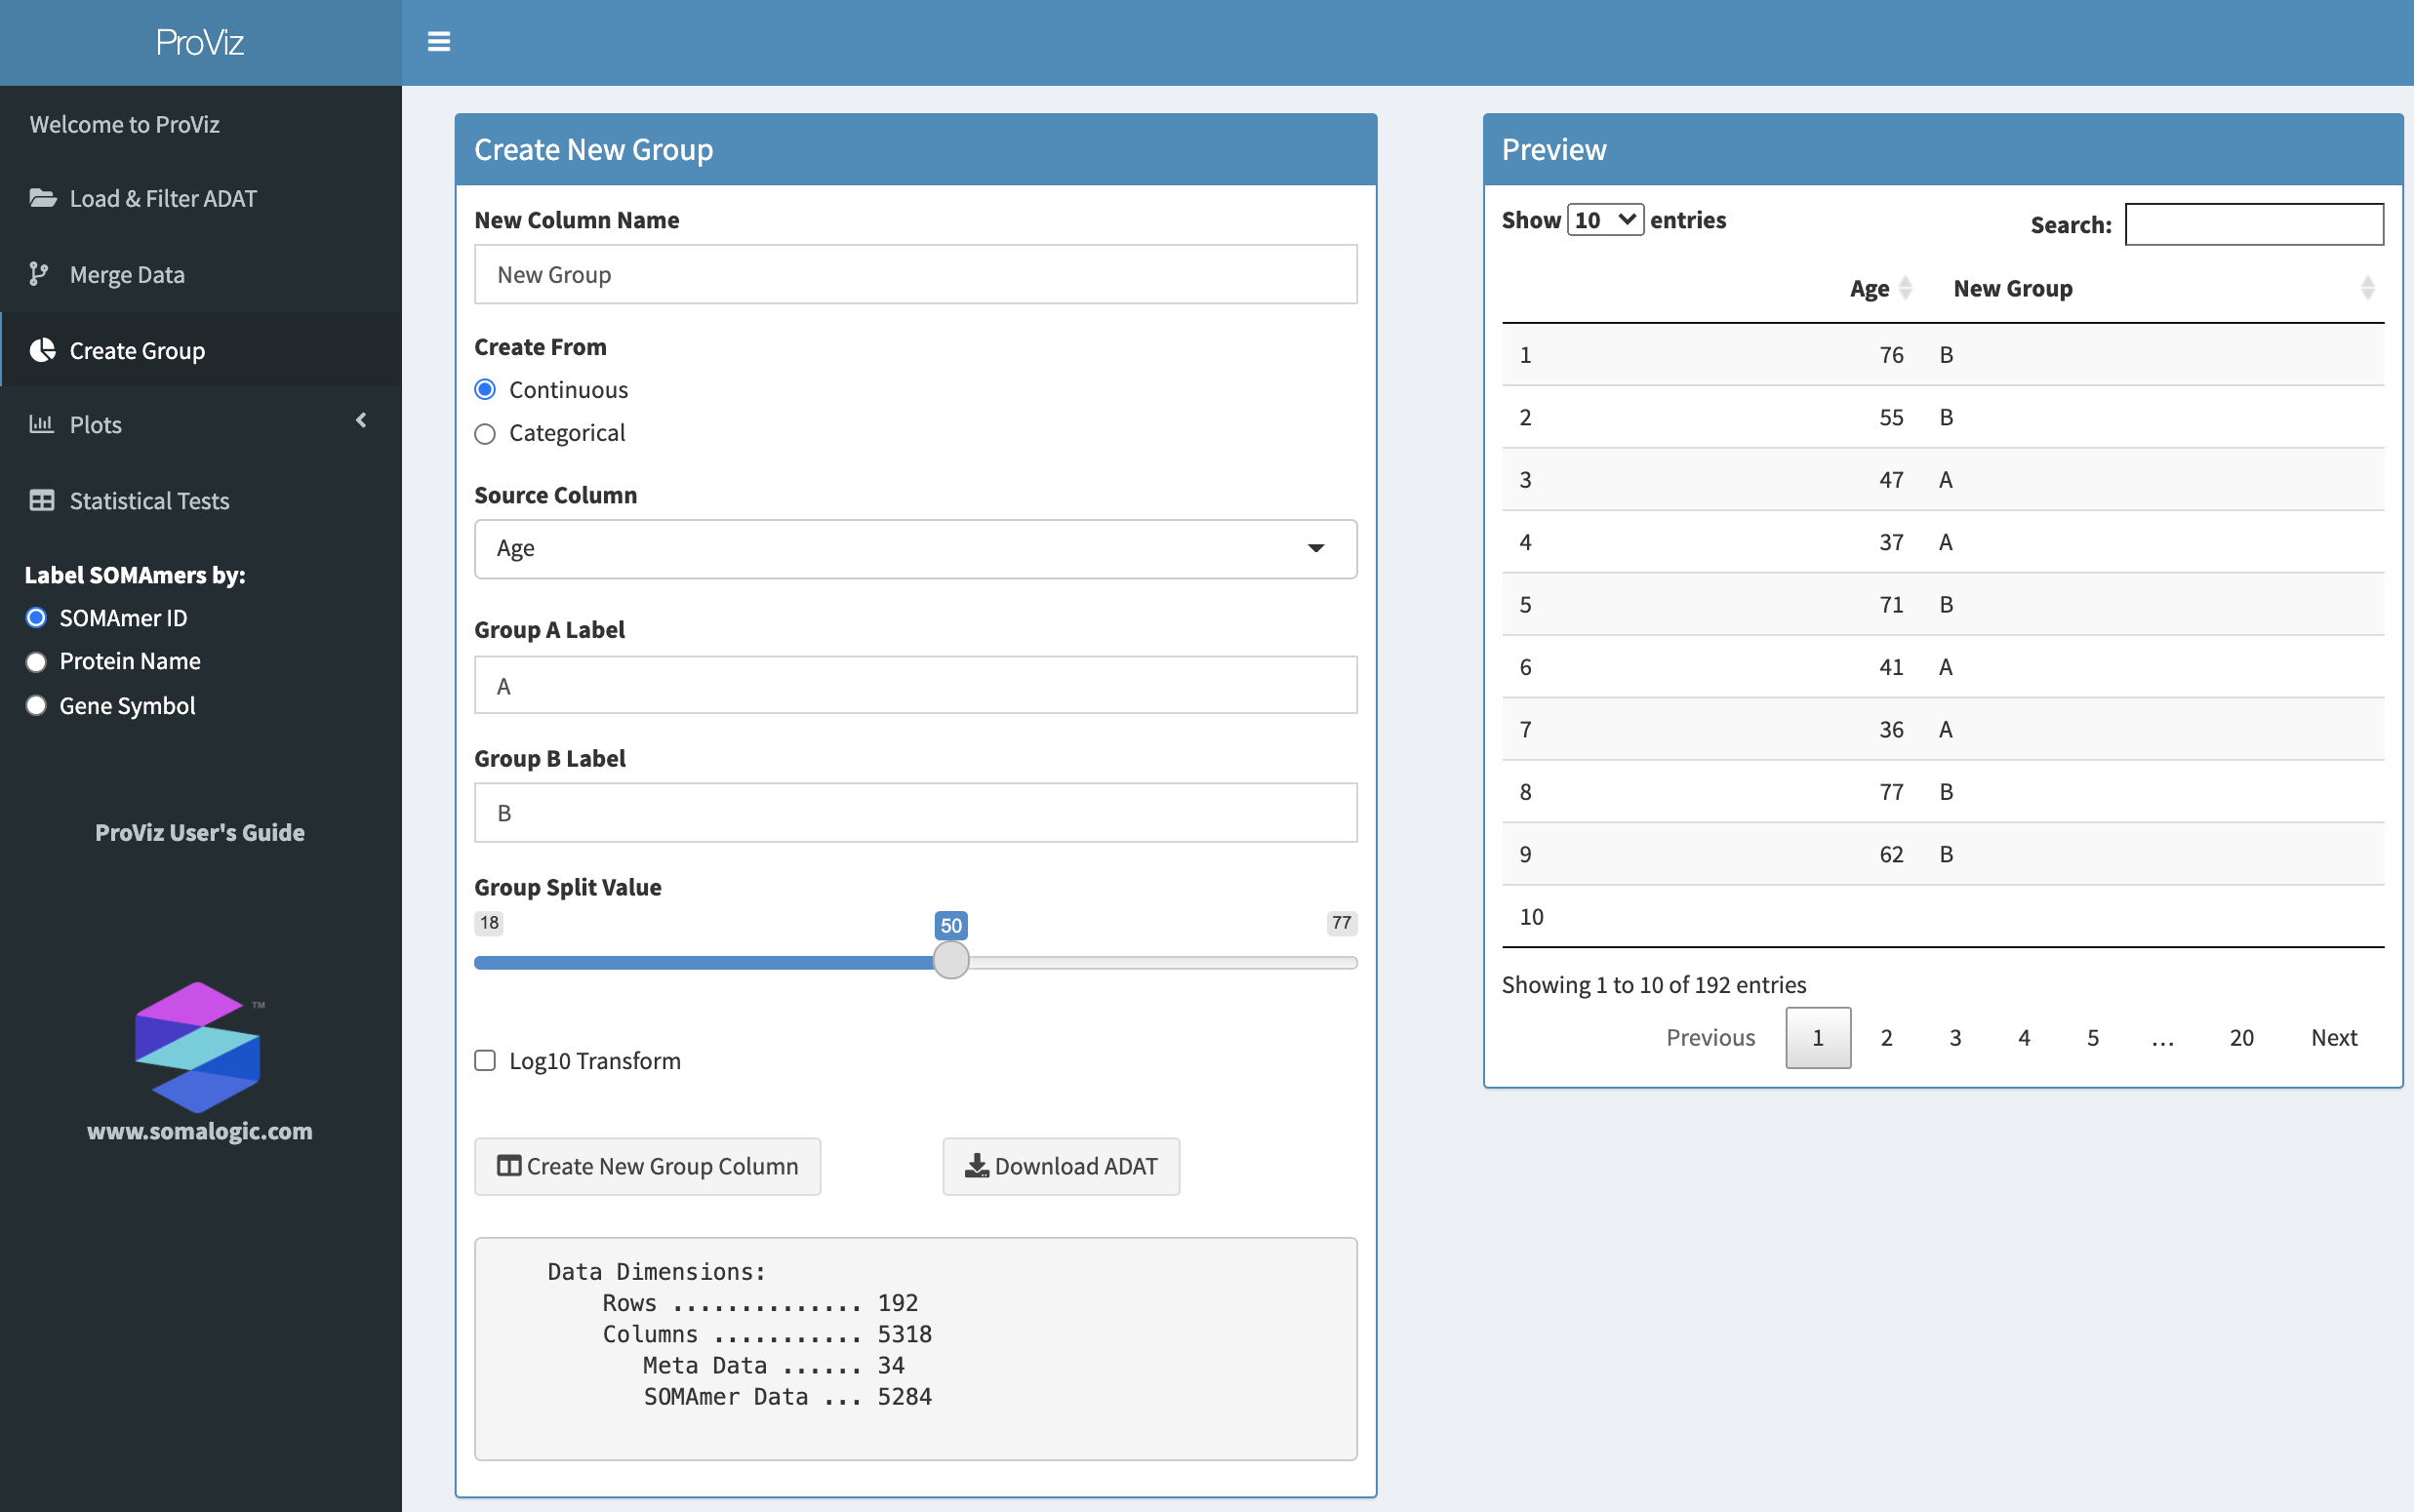
\includegraphics{images/CreateGroup.png}
\caption{The Create Group panel.}
\end{figure}

\hypertarget{creating-a-new-group-from-continuous-data}{%
\section{Creating a New Group from Continuous Data}\label{creating-a-new-group-from-continuous-data}}

\begin{figure}
\centering
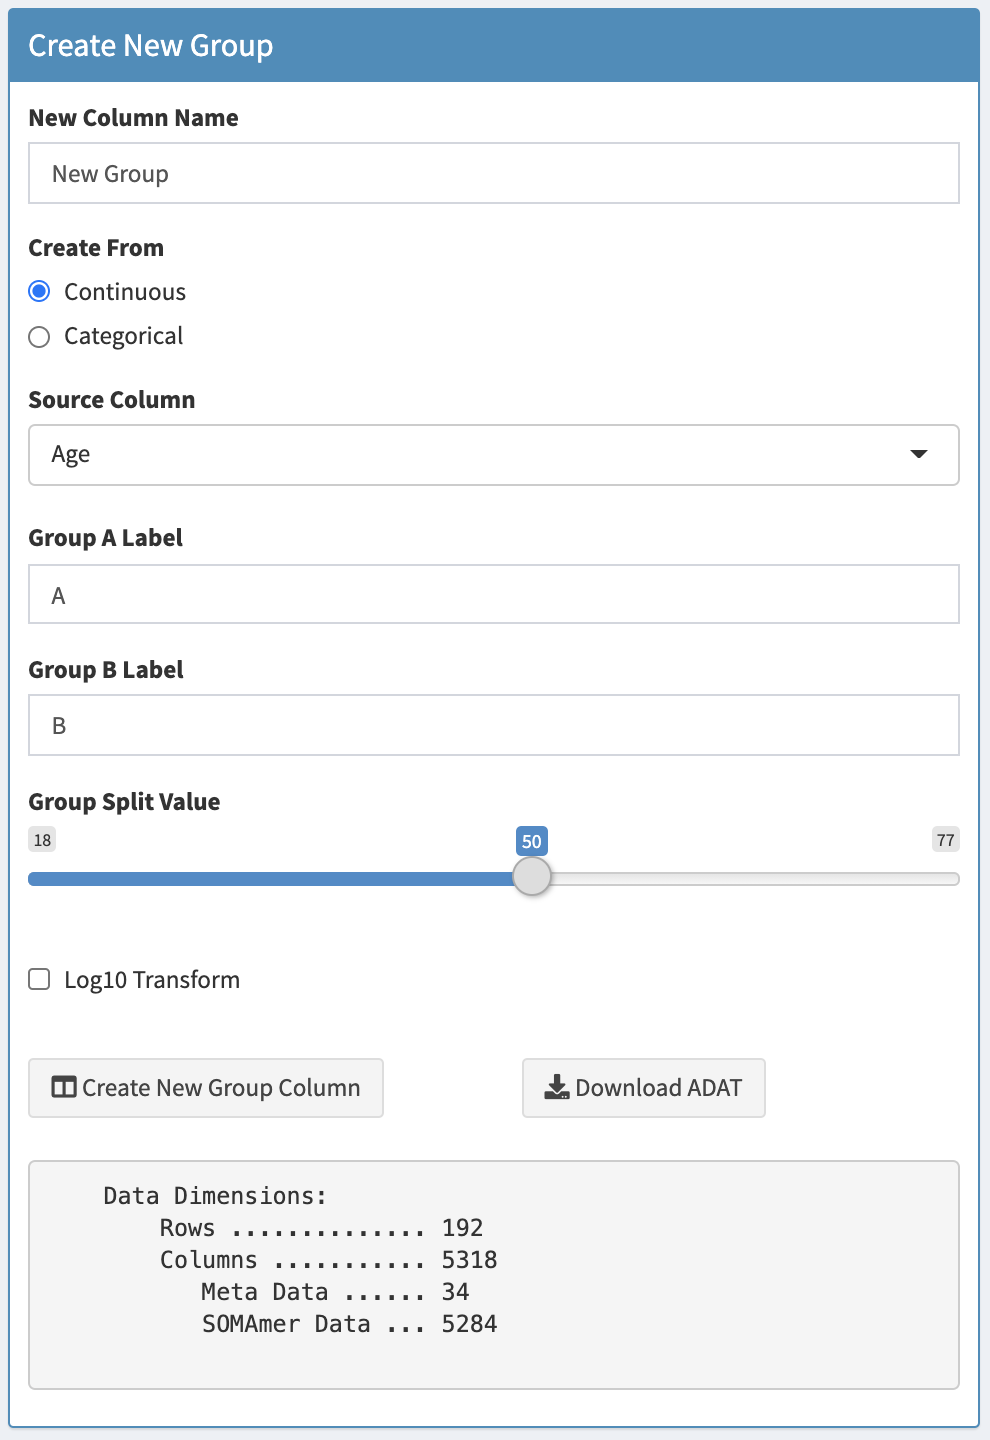
\includegraphics{images/CreateGroup_Continuous.png}
\caption{The Create New Group box with Continuous options selected.}
\end{figure}

\begin{itemize}
\tightlist
\item
  The column containing the new group variable can be named in the \textbf{New Column Name} box.\\
\item
  For splitting a continuous variable, select \emph{Continuous} from the \textbf{Create From} options.\\
\item
  The column containing the data to be split can be selected from the \textbf{Source Column} selection box.
\item
  Labels for the two groups are specified under \textbf{Group A Label} and \textbf{Group B Label}.
\item
  Adjust the \textbf{Group Split Value} slider to identify the split point for the data. Rows with values less than the chosen split will be given the label \emph{Group A} and rows with values greater than or equal to the chosen split will be given the label \emph{Group B}.
\item
  Data can be log10 transformed by selecting \textbf{Log10 Transform}.
\item
  A preview of the original data column and the newly created data column are shown at the right.
\item
  When ready to create the new group, press the \textbf{Create New Group Column} button, and the new column will be added to the ADAT.
\end{itemize}

In this example, a column titled \emph{New Group} will be created from the existing \emph{Age} column. Rows with values less than 50 will be given the label \emph{A} and values greater than or equal to 50 will be given the label \emph{B}.

\hypertarget{creating-a-new-group-from-categorical-data}{%
\section{Creating a New Group from Categorical Data}\label{creating-a-new-group-from-categorical-data}}

\begin{figure}
\centering
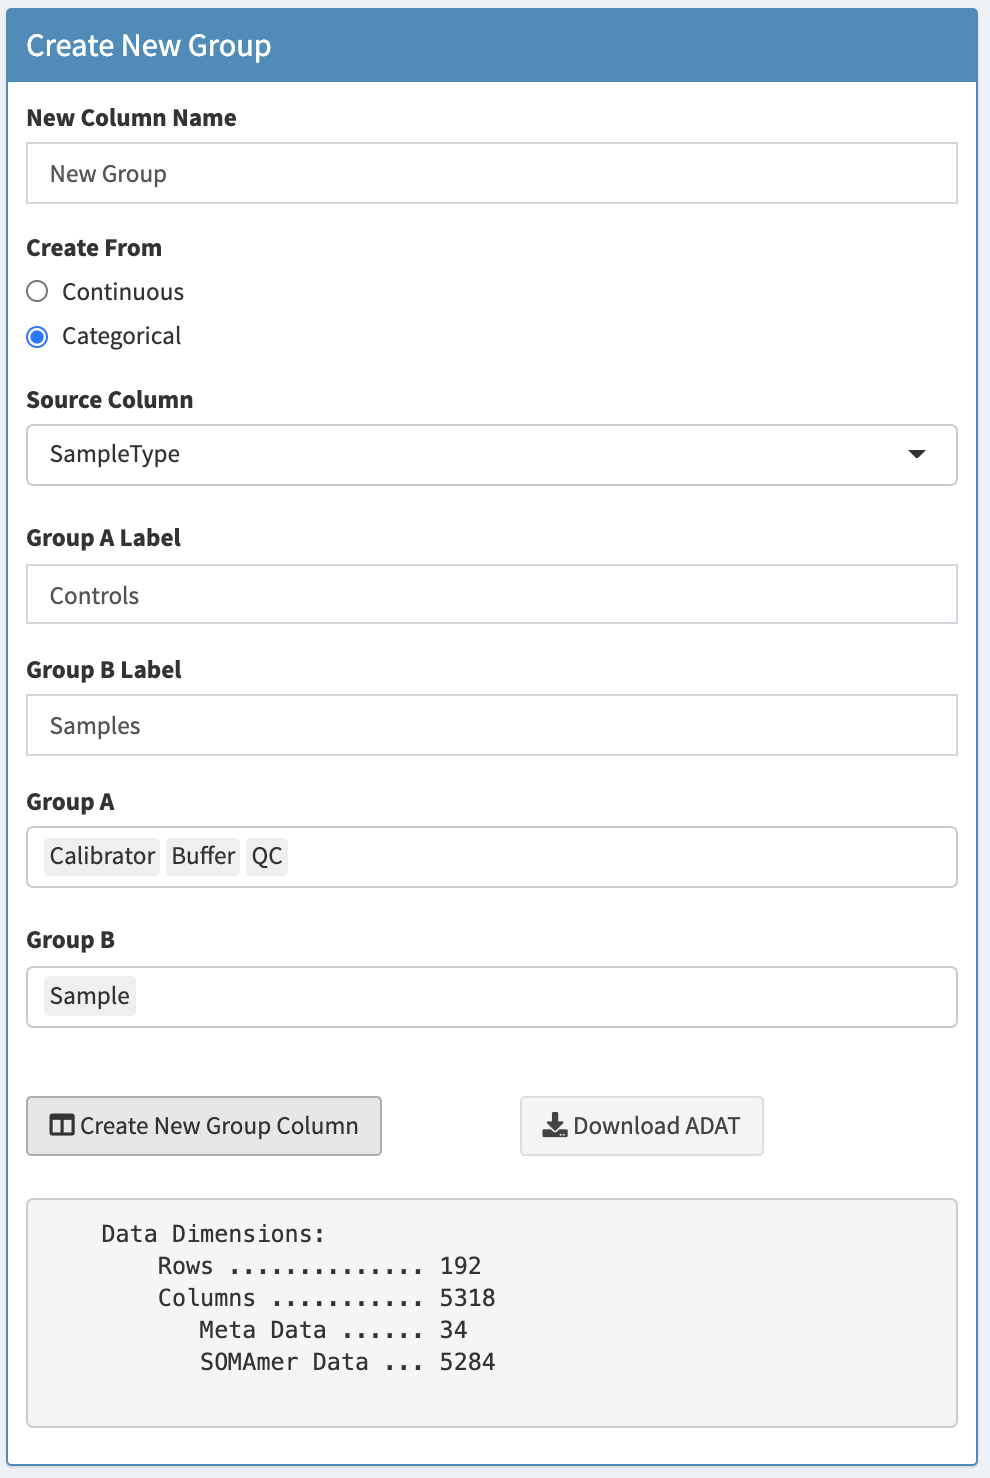
\includegraphics{images/CreateGroup_Categorical.png}
\caption{The Create New Group box with Categorical options selected.}
\end{figure}

\begin{itemize}
\tightlist
\item
  The column containing the new group variable can be named in the \textbf{New Column Name} box.\\
\item
  For splitting a categorical variable, select \emph{Categorical} from the \textbf{Create From} options.\\
\item
  Clicking on the \textbf{Group A} or \textbf{Group B} select boxes will show the categorical values available from the chosen column. Selections can be made by clicking on the categorical values desired for that group.
\item
  Labels for the two groups are specified under \textbf{Group A Label} and \textbf{Group B Label}.
\item
  A preview of the original data column and the newly created data column are shown at the right.
\item
  When ready to create the new group, press the \textbf{Create New Group Column} button, and the new column will be added to the ADAT.
\end{itemize}

In this example, a column titled \emph{New Group} will be created from the existing \emph{SampleType} column. Rows with values of \emph{Calibrator}, \emph{Buffer}, or \emph{QC} will be given the label \emph{Controls} and values of \emph{Sample} will be given the label \emph{Samples}. This will provide a useful label to distinguish between all controls and all clinical samples in the ADAT file.

\hypertarget{download-adat-2}{%
\section{Download ADAT}\label{download-adat-2}}

Once new groups have been created, a version of the ADAT can be downloaded by clicking the \textbf{Download ADAT} button. As this new ADAT file may be significantly modified relative to the original, ensure that a new, unique, descriptive file name is specified so that the original ADAT is not overwritten. Keeping good notes regarding the filtering operations is essential to recall how the ADAT was modified when it is returned to at a later date.

\hypertarget{plots}{%
\chapter{Plots}\label{plots}}

ProViz provides tools to dynamically create a variety of plots with custom options. Plots can be created using SomaScan Assay data as well as meta data in the ADAT or data imported in the \textbf{Merge Data} panel. Plot features such as titles, colors, and lines can be added and customized using selectable options in the ProViz plotting panels.

\hypertarget{plot-features}{%
\section{Plot Features}\label{plot-features}}

At any point during plotting, moving the mouse over the plot will show a toolbar a the top of the plot.

\begin{figure}
\centering

\includegraphics{images/modebar.png}
\caption{Plot toolbar}
\end{figure}

The icons from left to right provide the following features.

\begin{itemize}
\tightlist
\item
  download as PNG - saves the image to a file
\item
  zoom - when selected, the plot can be zoomed by clicking and dragging the mouse
\item
  pan - when selected, the plot can be moved by clicking a dragging
\item
  zoom in - zooms into the plot, keeping the current center
\item
  zoom out - zooms into the plot, keping the current center
\item
  autoscale - resets the coordinates of the plot if it has been zoomed or panned (similar to reset axes, below)
\item
  reset axes - resets coordinates of the plot if it has been zoomed or panned (similar to autoscael, above)
\item
  toggle spike lines - when selected, hovering over points on the graph will also include lines from teh point to the axes
\item
  show closest data on hover - only informaiton about the closest data point will be shown when the point is hovered over
\item
  compare data on hover - if multiple points are plotted at the same location, data for all points will be shown
\item
  Plotly icon - a link to the Plotly website. Plotly is the tool used by ProViz to produce graphs.
\end{itemize}

\hypertarget{dynamic-plot-interactions}{%
\section{Dynamic Plot Interactions}\label{dynamic-plot-interactions}}

At any point during plotting, the plots provide dynamic interaction capabilities. Hovering on the plotted elements themselves, such as boxes in a box plot or points in any plot, provides additional information about the samples corresponding to that plotting element. Plots can be zoomed or panned by clicking and dragging - see the details above in \textbf{Plot Features}.

\hypertarget{boxplots}{%
\section{Boxplots}\label{boxplots}}

\begin{figure}
\centering
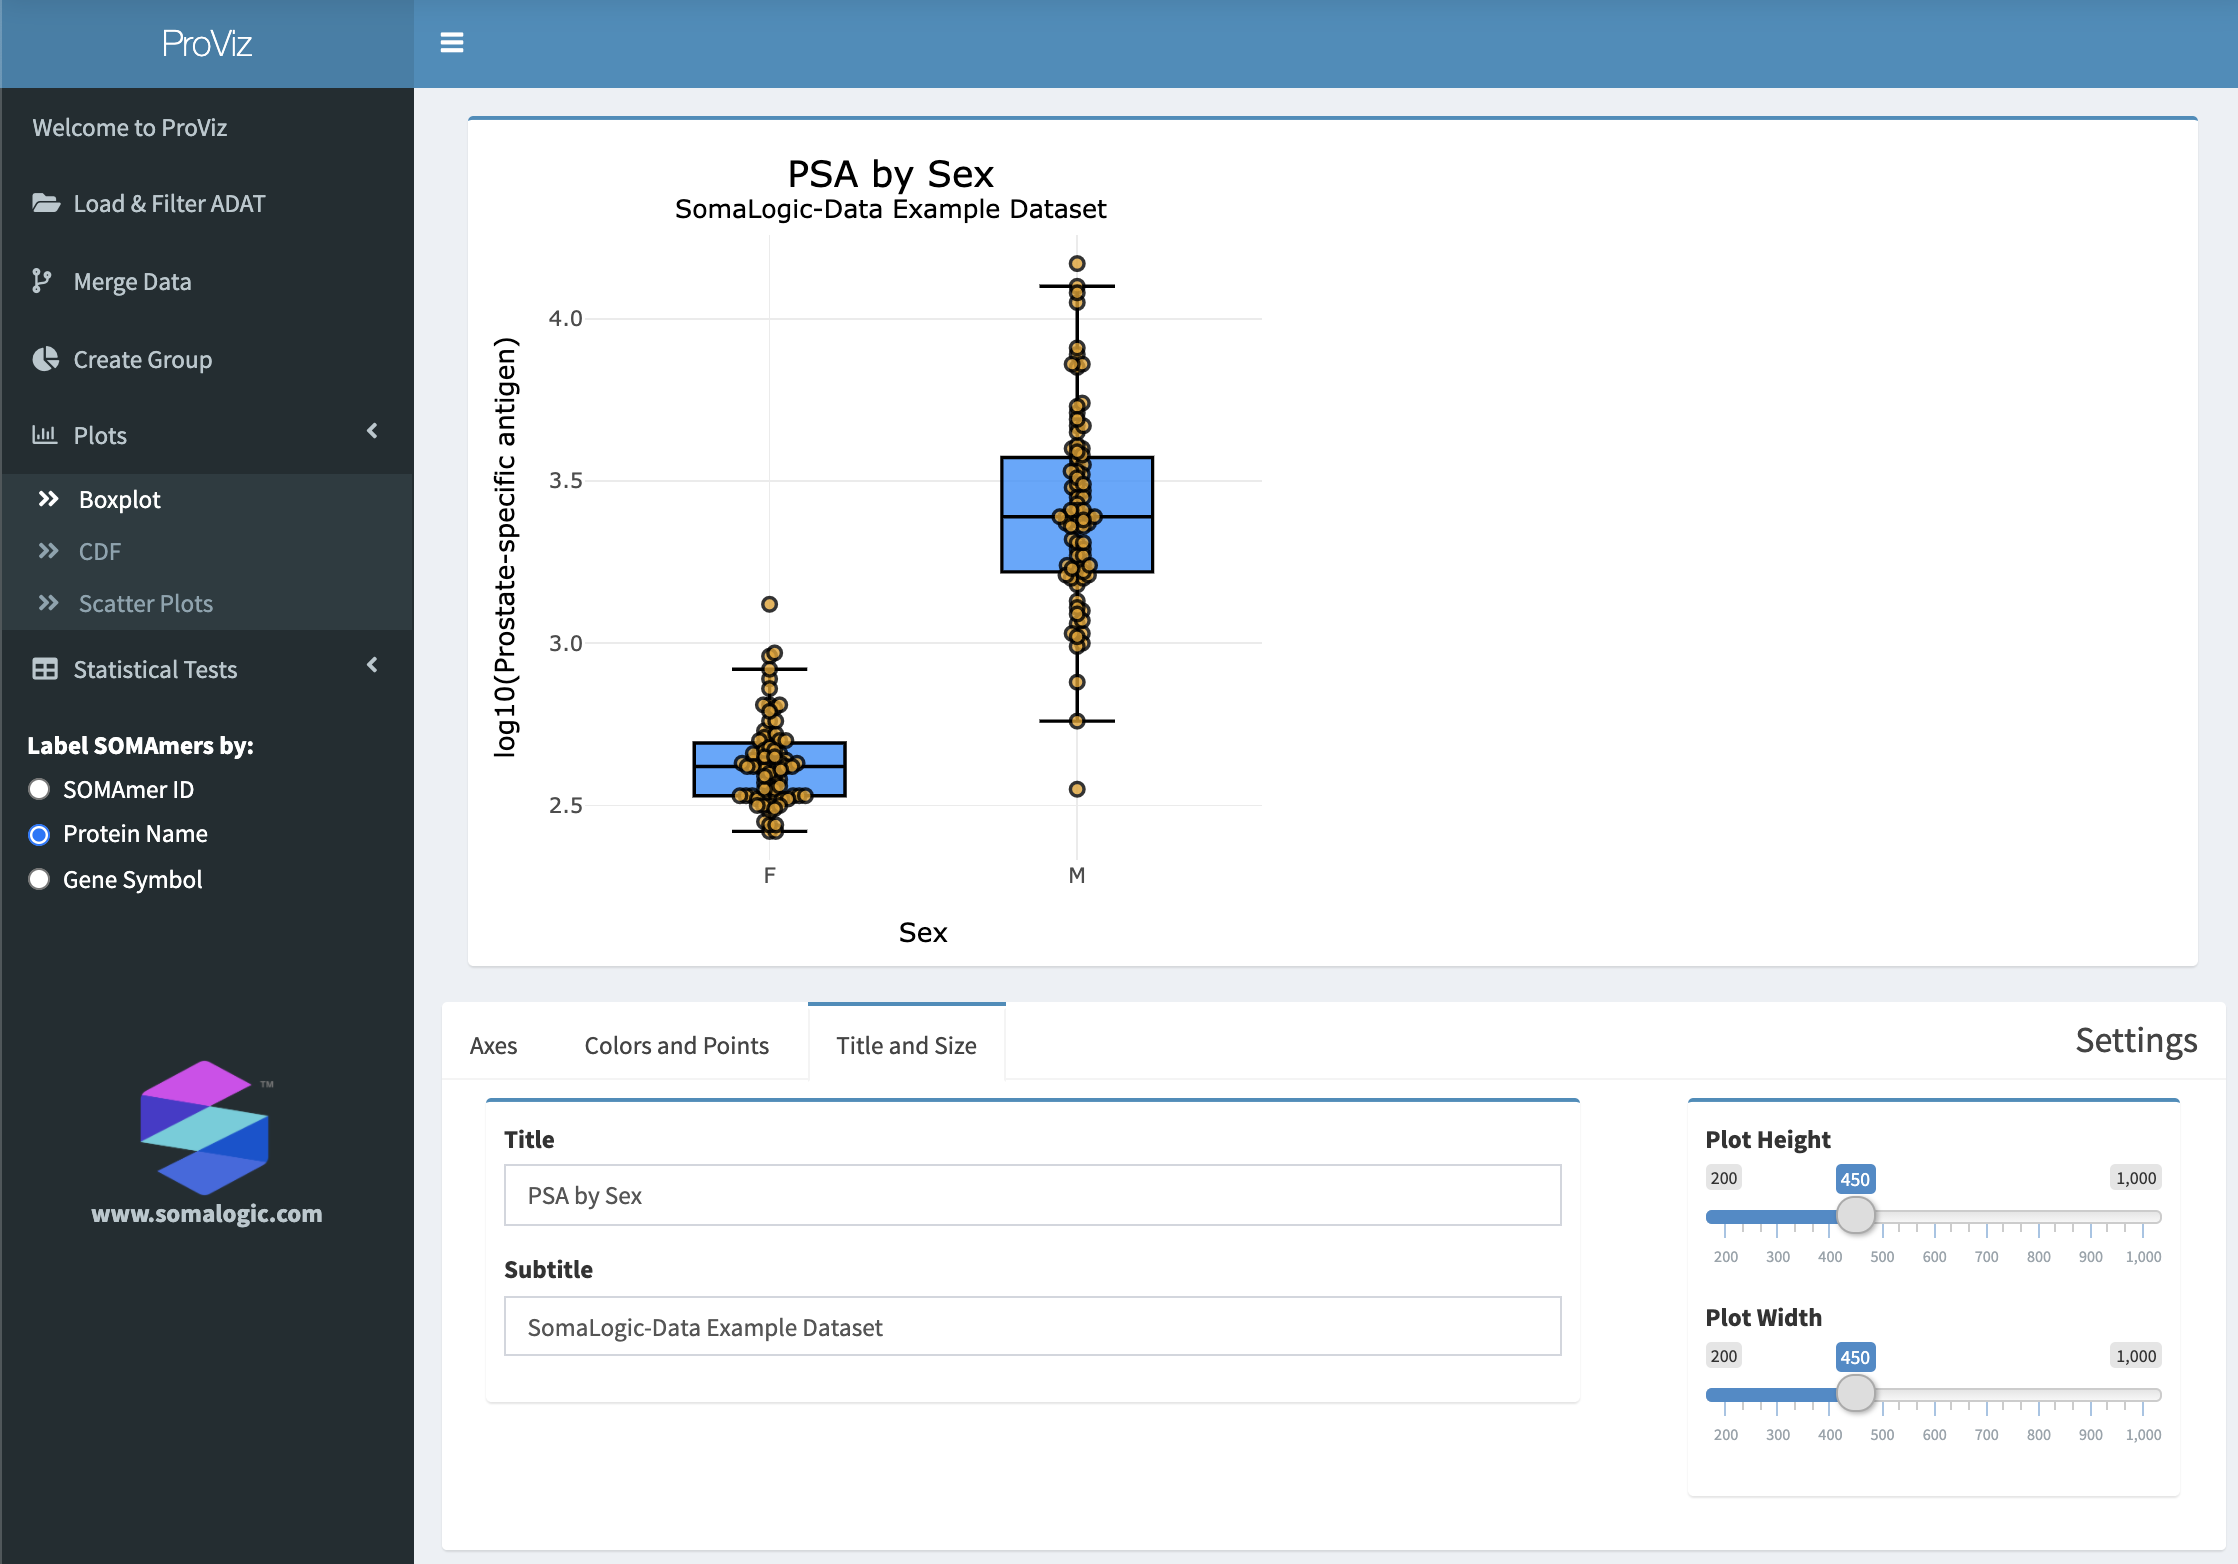
\includegraphics{images/BoxPlot_Panel.png}
\caption{The Boxplot panel with a customized plot.}
\end{figure}

\hypertarget{axes}{%
\subsection{Axes}\label{axes}}

\begin{figure}
\centering
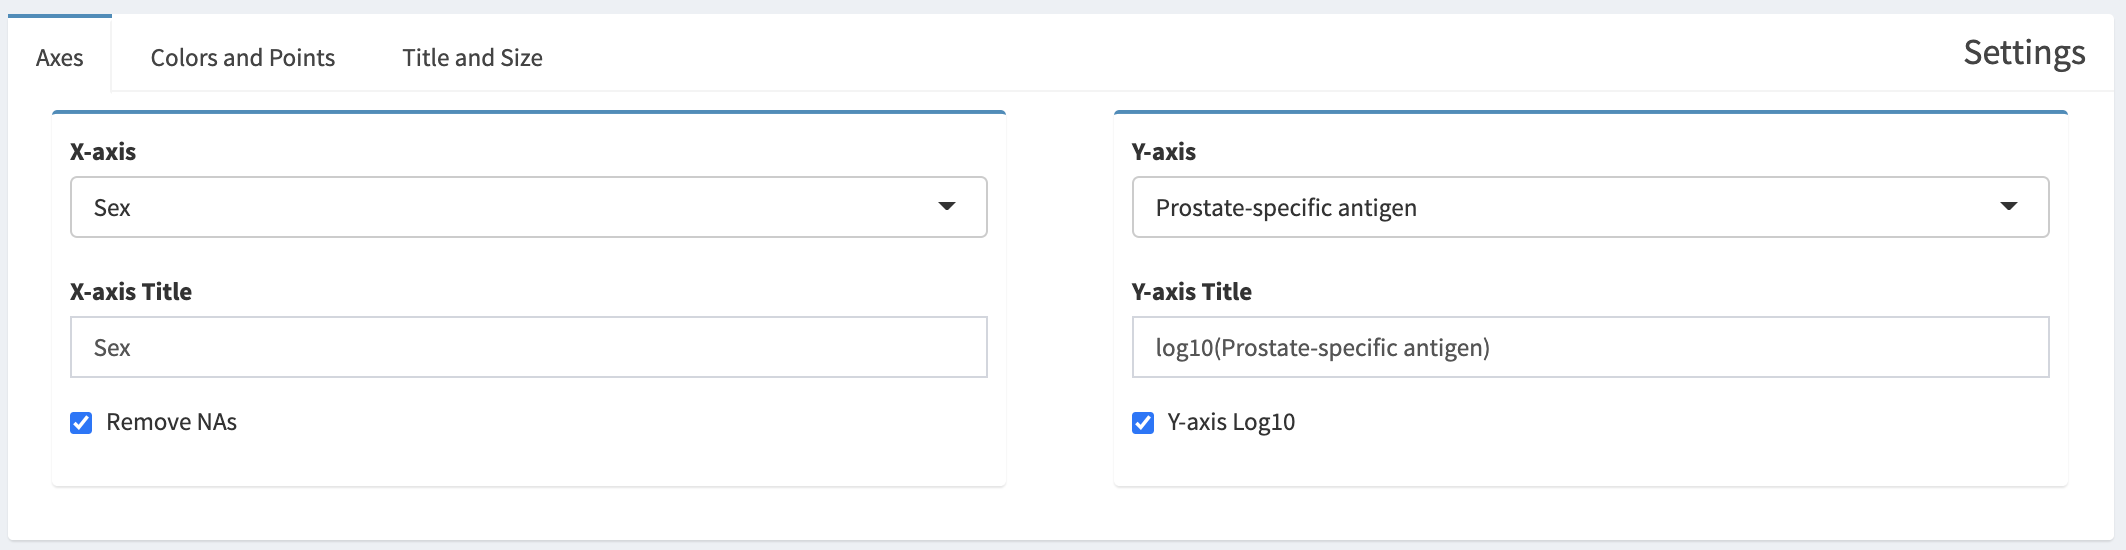
\includegraphics{images/Boxplot_Axes.png}
\caption{The Axes tab in the Plot Settings box.}
\end{figure}

A categorical variable that defines the boxes in the boxplot can be selected from the \textbf{X-axis} select box. If the categorical variable has missing values (NAs), those can be removed by selected \textbf{Remove NAs}.

A continuous variable can be selecged from the \textbf{Y-axis} select box. The continuous variable can be transformed by log10 by selecting \textbf{Y-axis Log10}.

\hypertarget{colors-and-points}{%
\subsection{Colors and Points}\label{colors-and-points}}

\begin{figure}
\centering
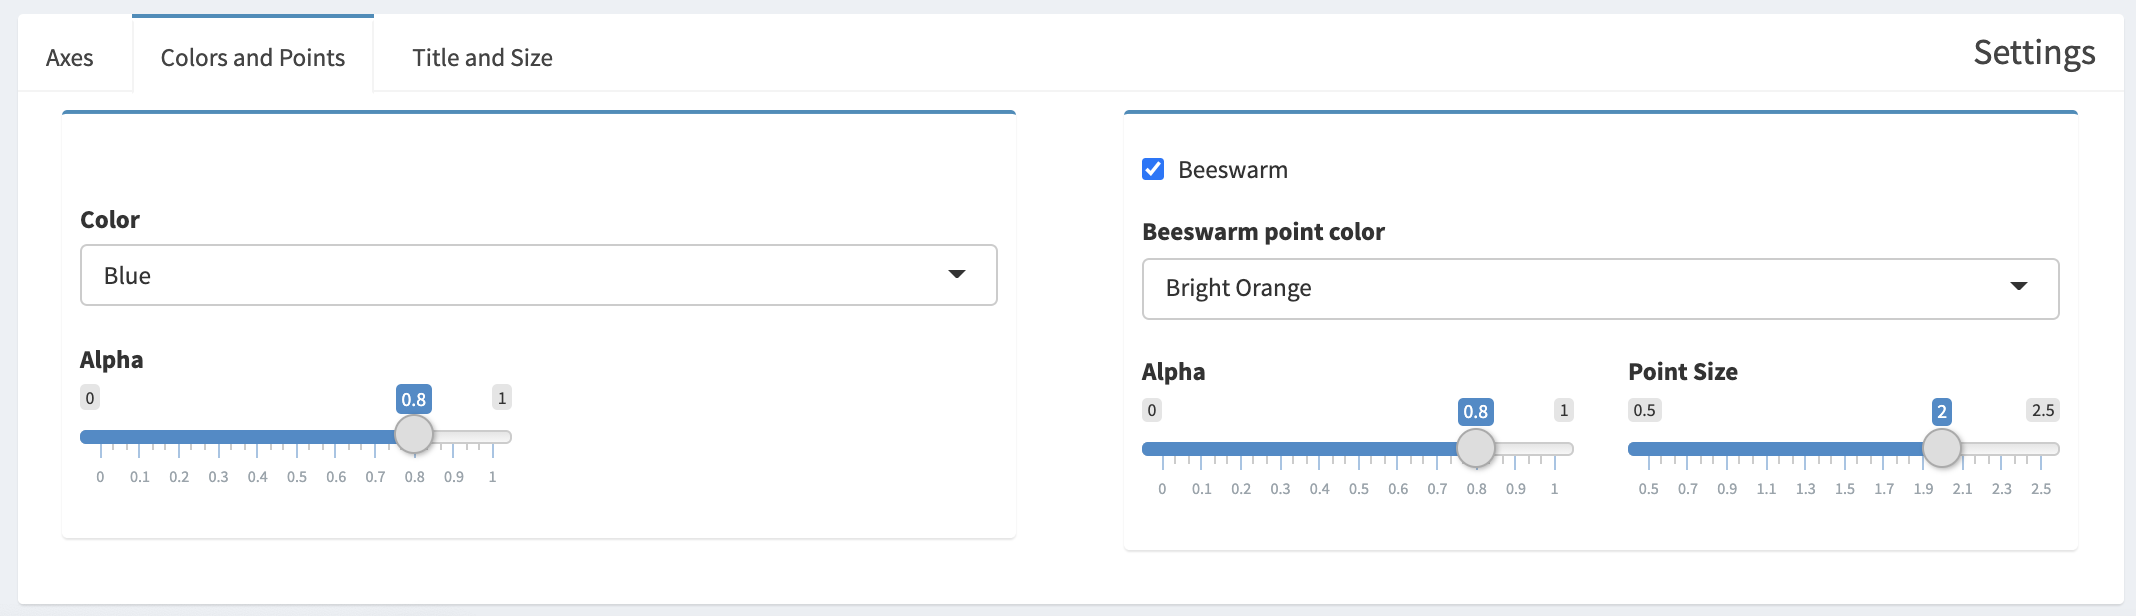
\includegraphics{images/Boxplot_ColorsPoints.png}
\caption{The Colors and Points tabs in the Plot Settings box.}
\end{figure}

Colors of boxes can be customized by selecting from the \textbf{Color} select box, and the degree of transparency can be adjusted with the \textbf{Alpha} slider on the left.

Individual points for each sample can be displayed by selected \textbf{Beeswarm}. Colors of the points can be customized by selecting a color from \textbf{Beeswarm point color} and the transparency can be adjusted with the \textbf{Alpha} slider on the right. The size of the points can be adjusted with the \textbf{Point Size} slider.

\hypertarget{title-and-size}{%
\subsection{Title and Size}\label{title-and-size}}

\begin{figure}
\centering
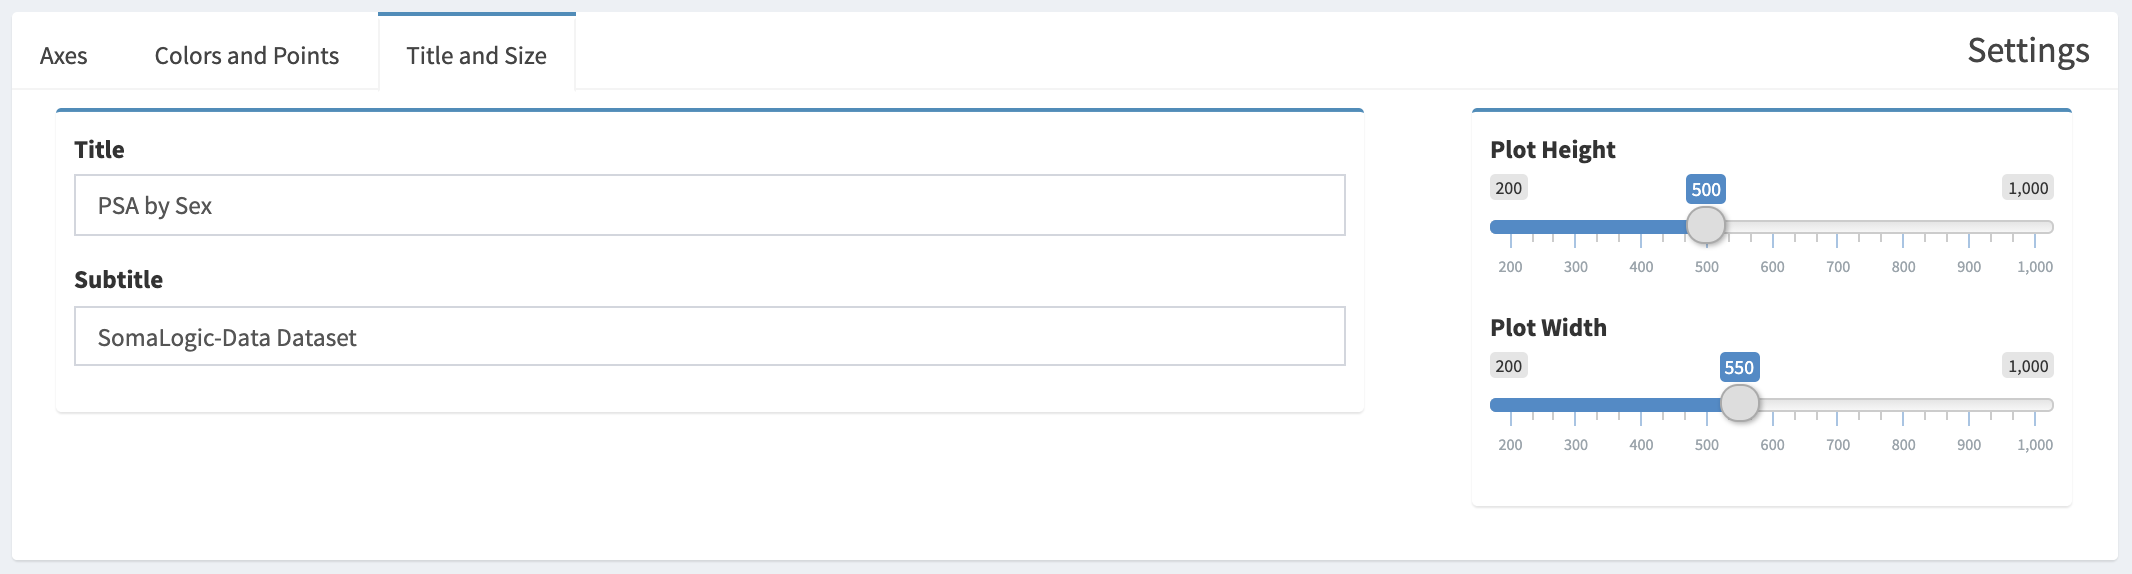
\includegraphics{images/Boxplot_TitleSize.png}
\caption{The Title and Size tab in the Plot Settings box.}
\end{figure}

A title and subtitle can be added to the plot by entering text into the \textbf{Title} and \textbf{Subtitle} boxes. The plot size can be adjusted using the \textbf{Plot Height} and \textbf{Plot Width} sliders.

\hypertarget{cdf-plots}{%
\section{CDF Plots}\label{cdf-plots}}

\begin{figure}
\centering
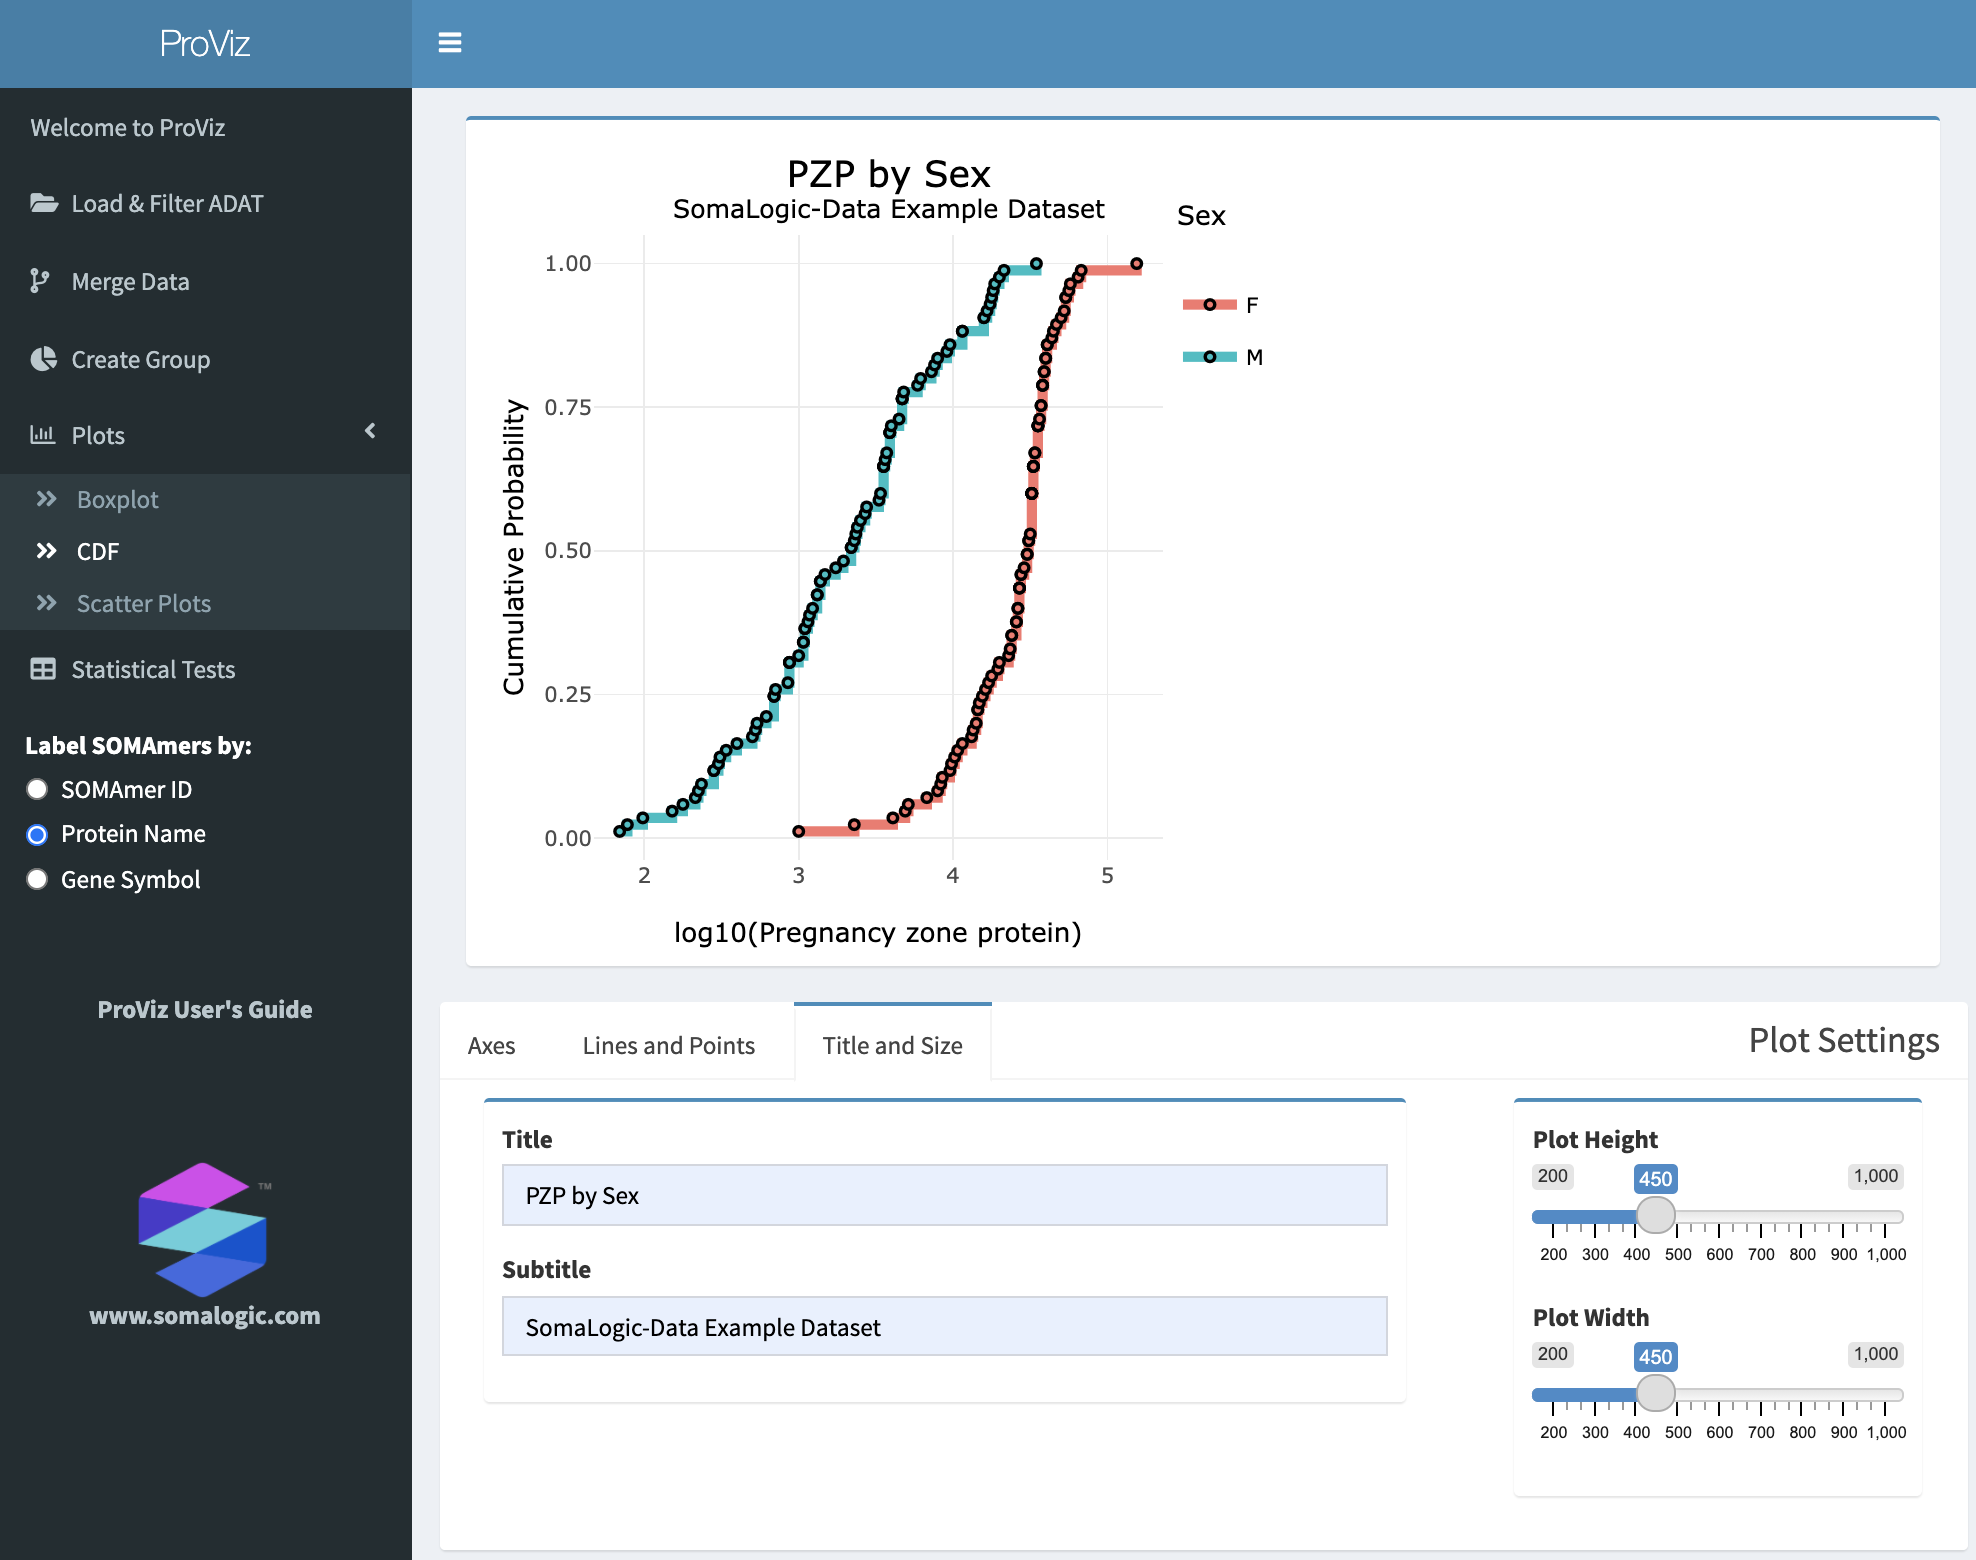
\includegraphics{images/CDF_Panel.png}
\caption{The CDF panel with a customized plot.}
\end{figure}

\hypertarget{axes-1}{%
\subsection{Axes}\label{axes-1}}

\begin{figure}
\centering
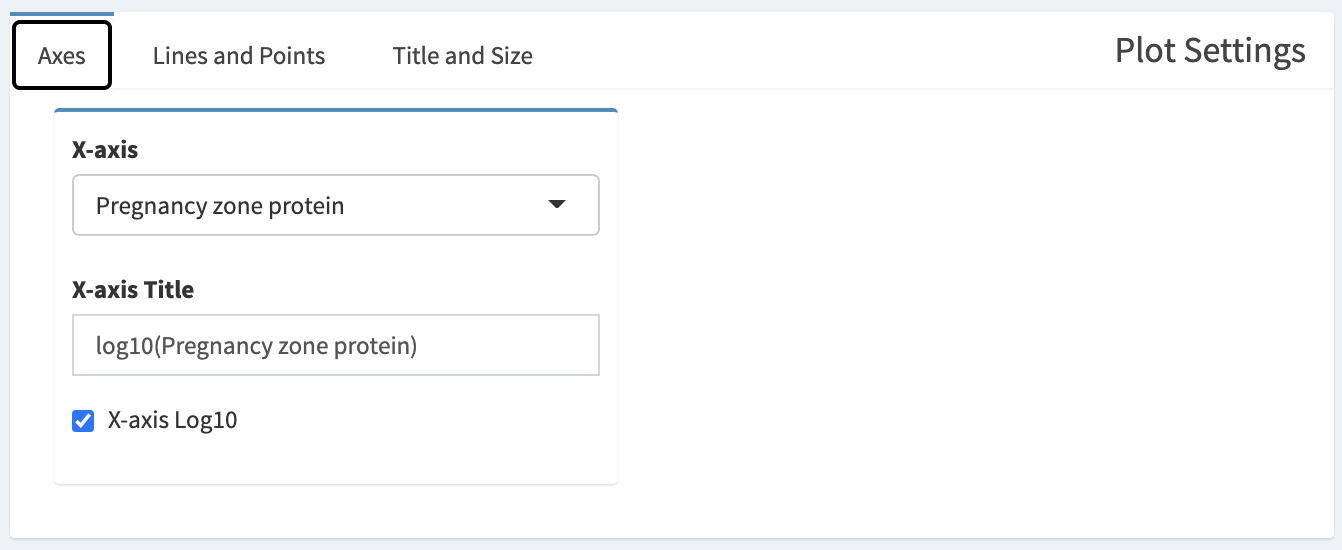
\includegraphics{images/CDF_Axes.png}
\caption{The Axes tab in the Plot Settings box.}
\end{figure}

A continuous variable can be selected from the \textbf{X-axis} select box. The continuous variable can be log10 transformed by selecting \textbf{X-axis Log10}.

\hypertarget{lines-and-points}{%
\subsection{Lines and Points}\label{lines-and-points}}

\begin{figure}
\centering
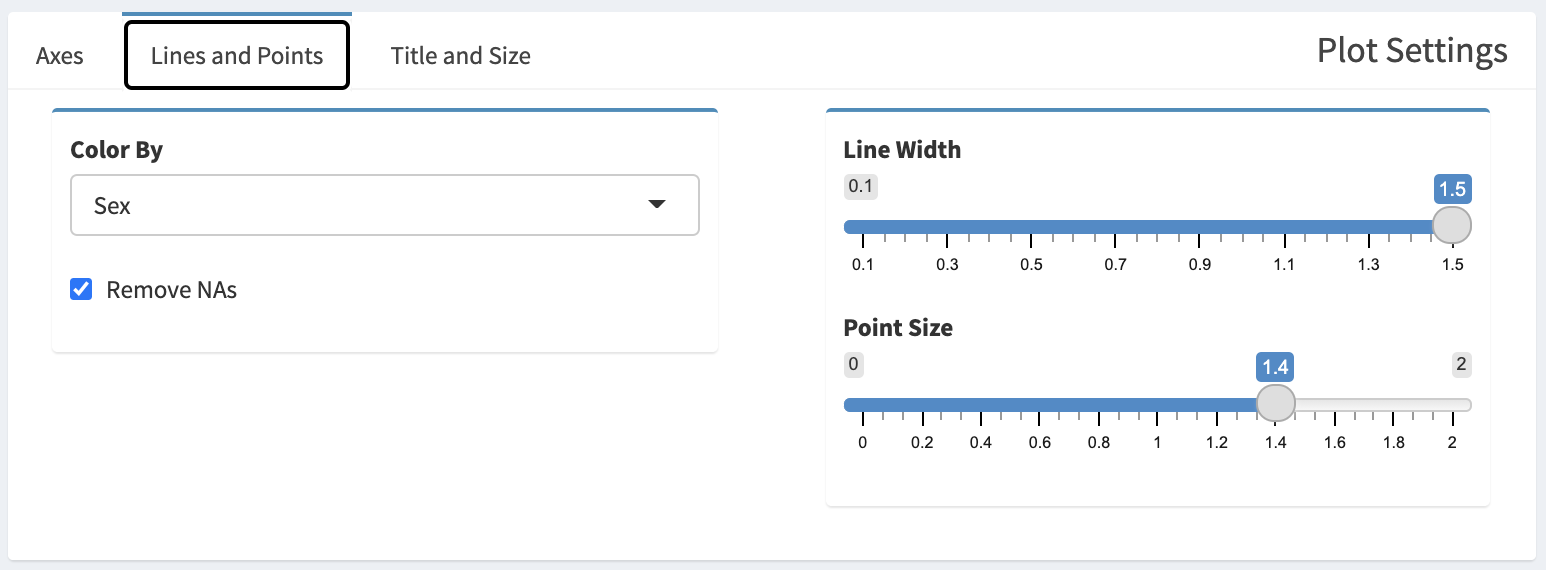
\includegraphics{images/CDF_LinesPoints.png}
\caption{The Lines and Points tab in the Plot Settings box.}
\end{figure}

A categorical variable can be selected from the \textbf{Color By} select box, which will produce one CDF for each category in that variable. If there are NAs for some samples, a CDF will also be produced for NA-containing set, or it can be removed by selecting \textbf{Remove NAs}. Line width can be adjusted using the \textbf{Line Width} slider, and point sizes can be adjusted with the \textbf{Point Size} slider. If the \textbf{Point Size} slider is set to \emph{0}, points will be removed from the plot.

\hypertarget{title-and-size-1}{%
\subsection{Title and Size}\label{title-and-size-1}}

\begin{figure}
\centering
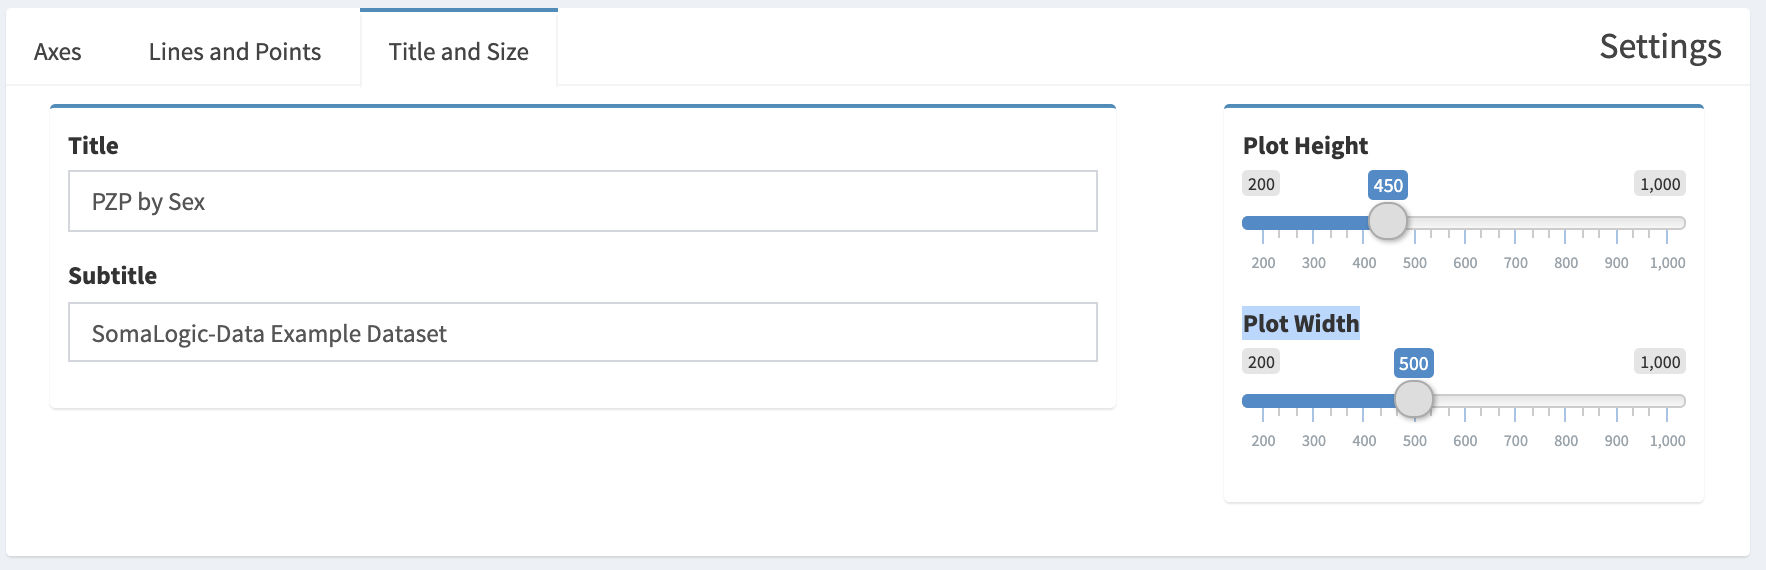
\includegraphics{images/CDF_TitleSize.png}
\caption{The Title and Size tab in the Plot Settings box.}
\end{figure}

A title and subtitle can be added to the plot by entering text into the \textbf{Title} and \textbf{Subtitle} boxes. The plot size can be adjusted using the \textbf{Plot Height} and \textbf{Plot Width} sliders.

\hypertarget{scatter-plots}{%
\section{Scatter Plots}\label{scatter-plots}}

\begin{figure}
\centering
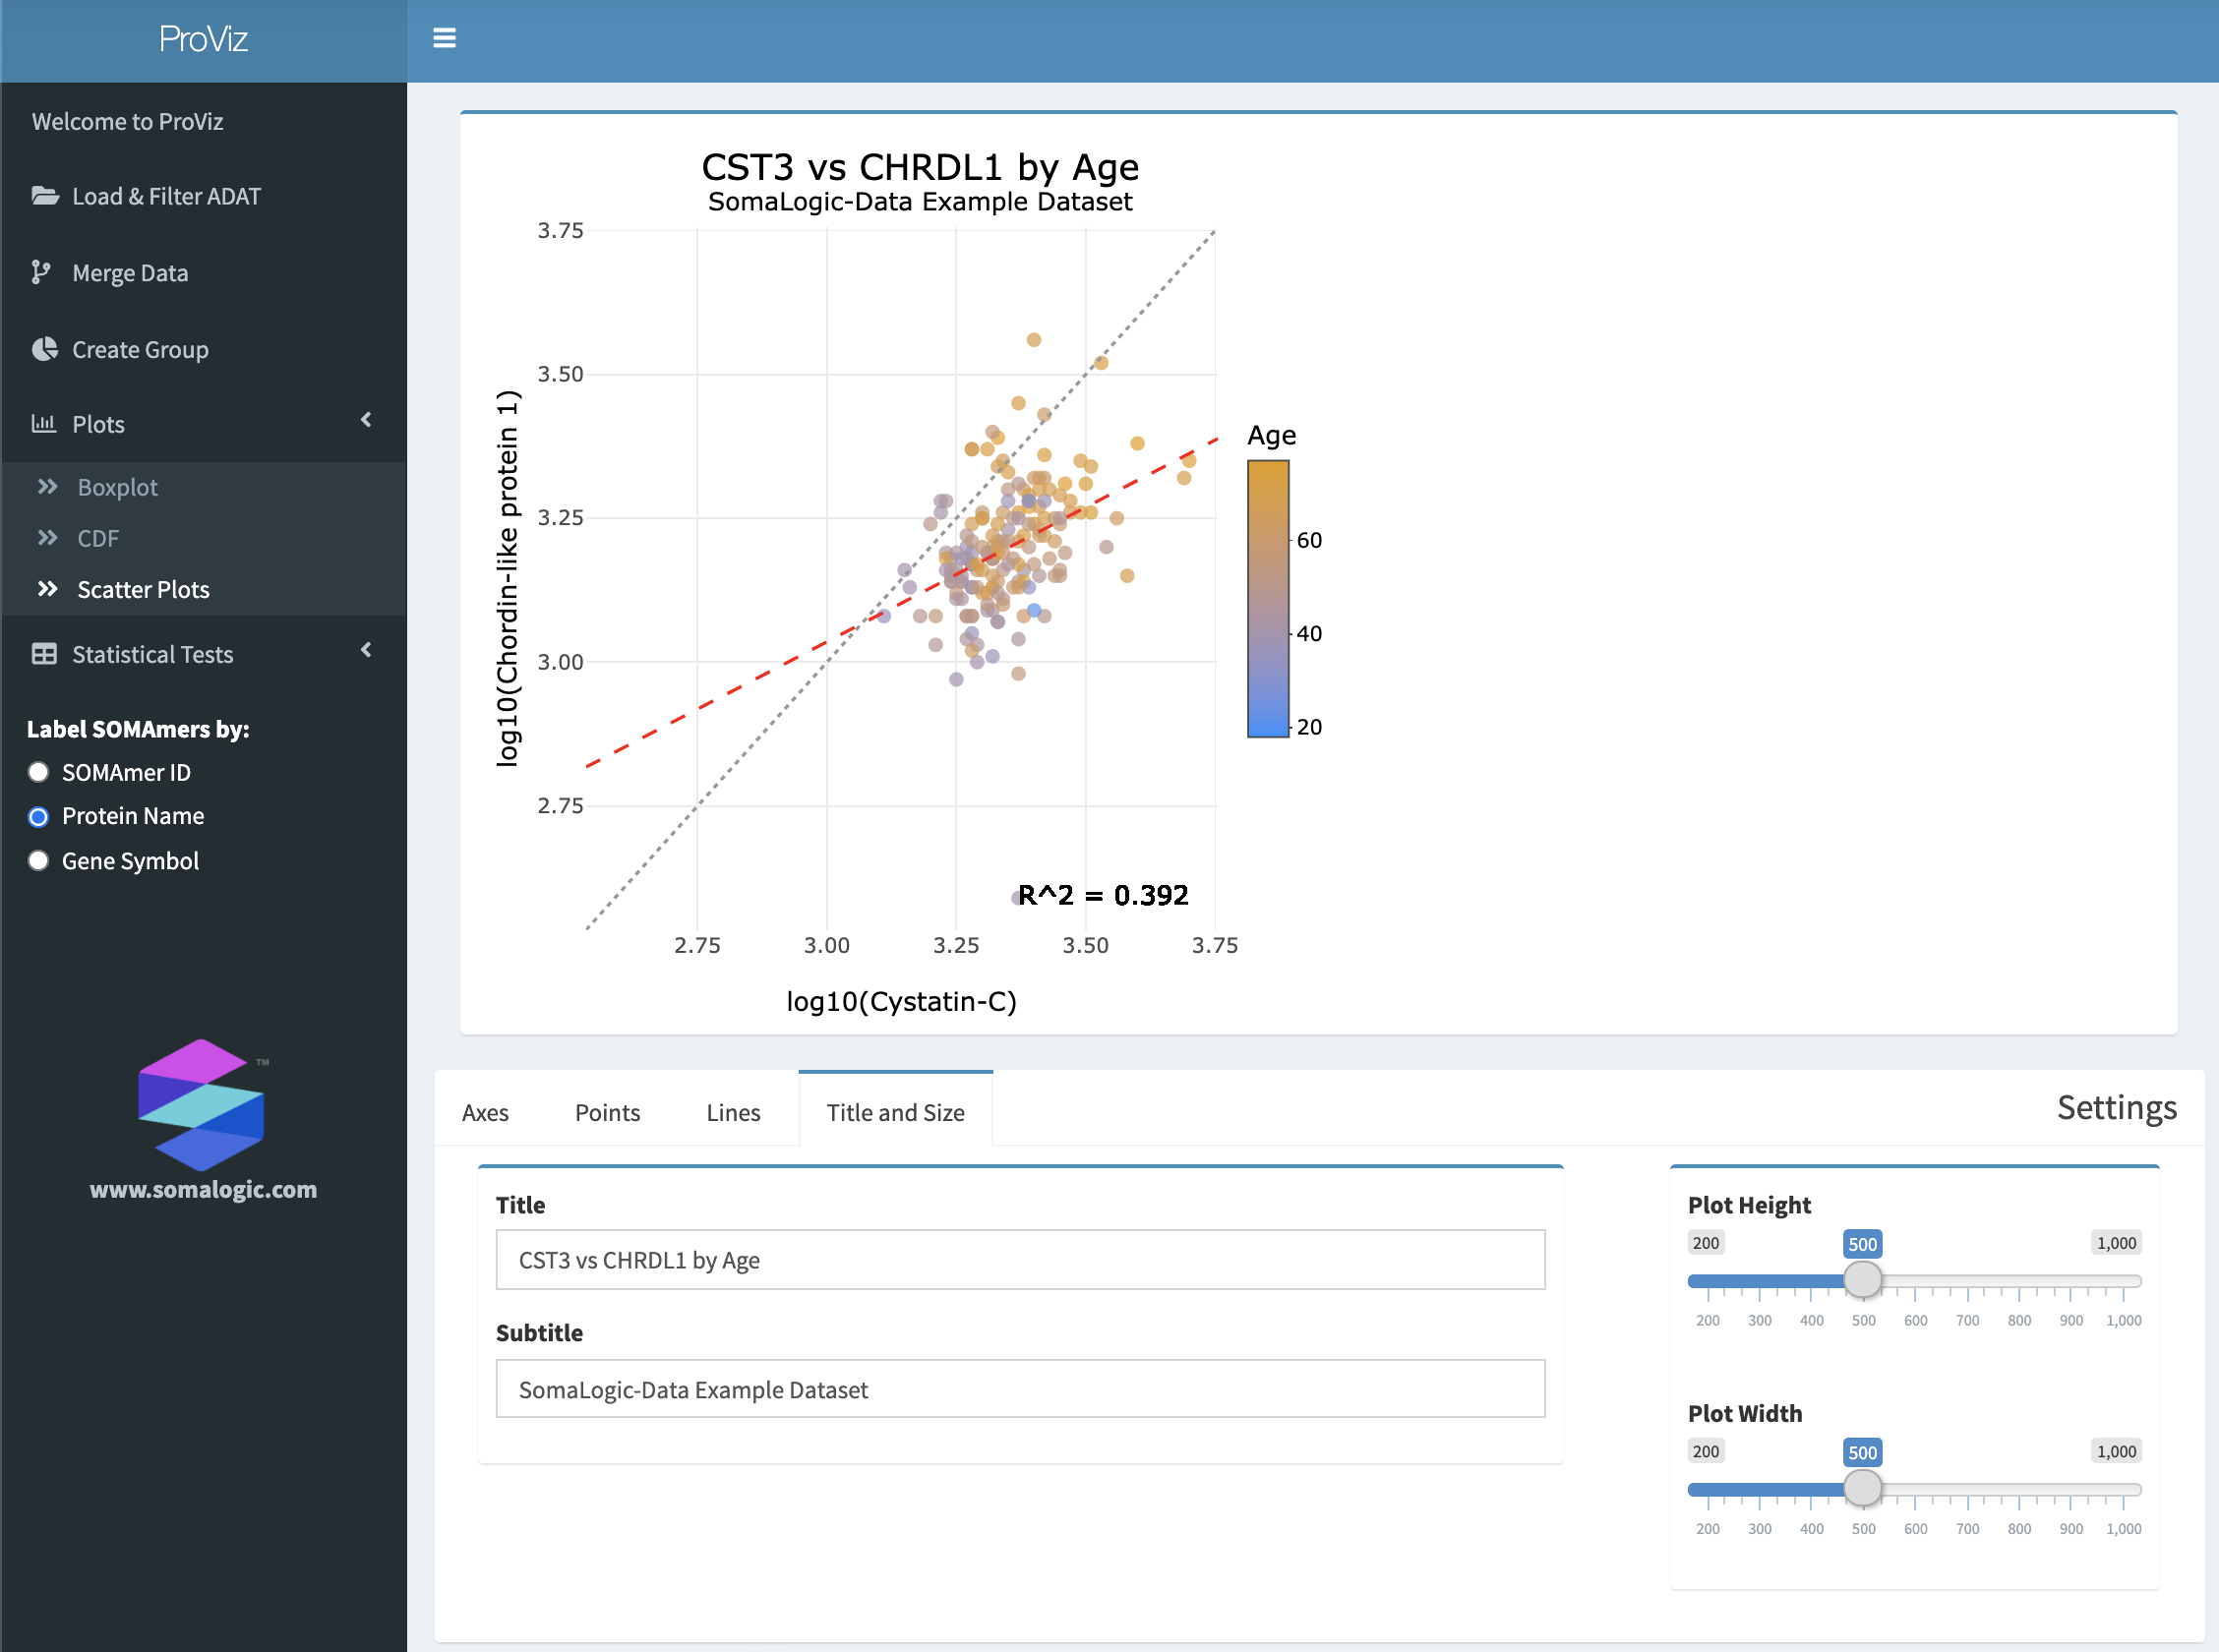
\includegraphics{images/Scatter_Panel.png}
\caption{The Scatter Plot panel with a customized plot.}
\end{figure}

\hypertarget{axes-2}{%
\subsection{Axes}\label{axes-2}}

\begin{figure}
\centering
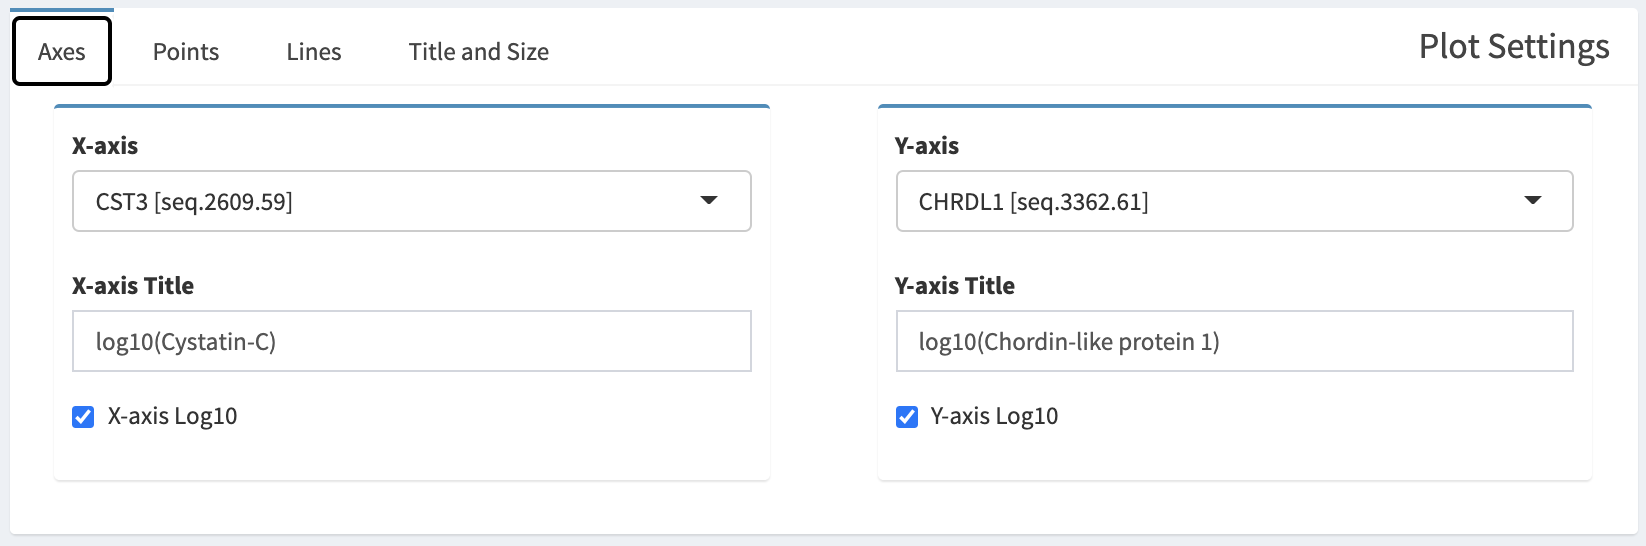
\includegraphics{images/Scatter_Axes.png}
\caption{The Axes tab in the Plot Settings box.}
\end{figure}

To set the X- and Y-axes, select continuous variables from the \textbf{X-axis} and \textbf{Y-axis} select boxes. Selecting \textbf{X-axis Log10} or \textbf{Y-axis Log10} will log10 transform the data for that axis.

\hypertarget{points}{%
\subsection{Points}\label{points}}

\begin{figure}
\centering
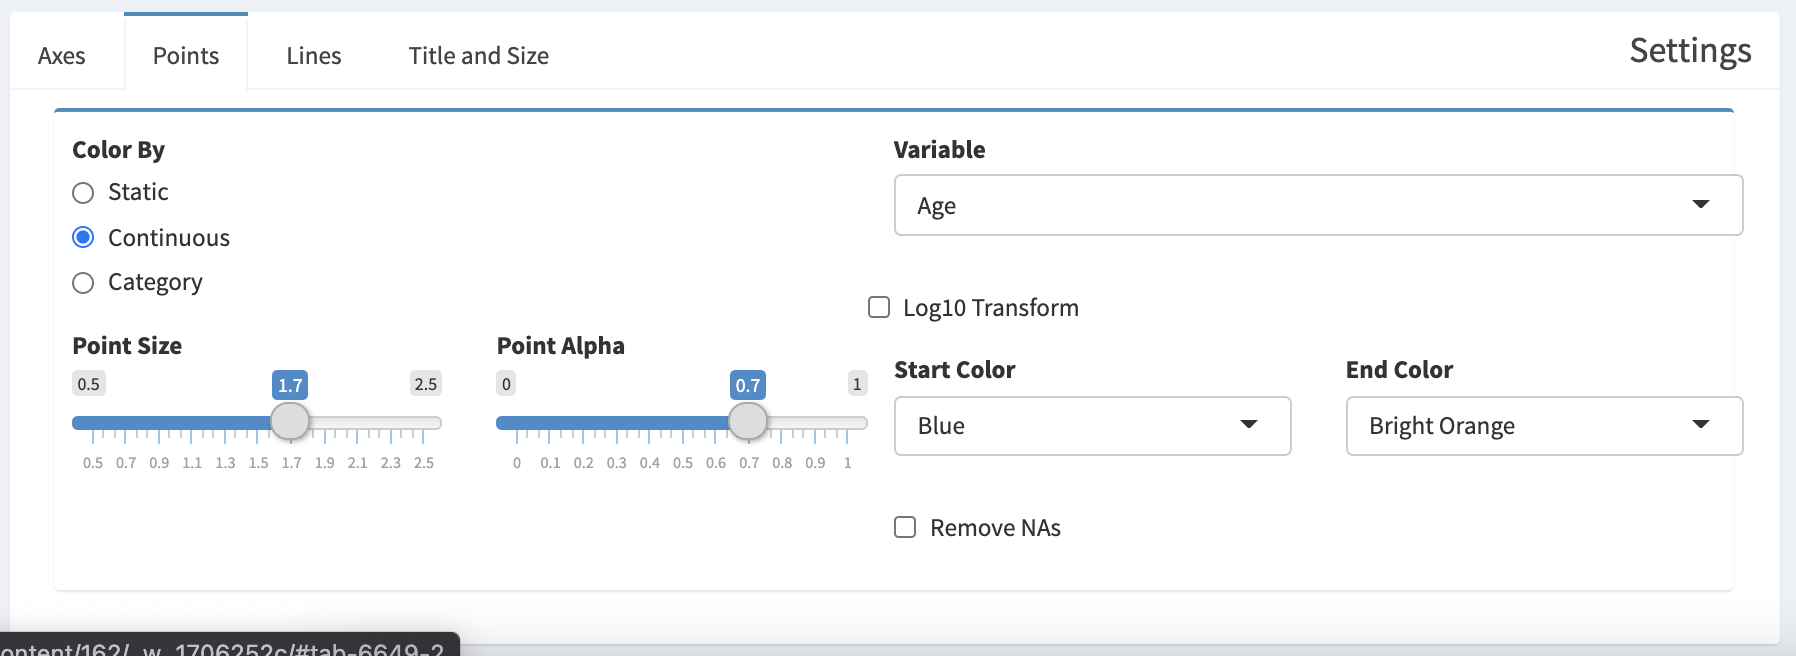
\includegraphics{images/Scatter_Points.png}
\caption{The Points tab in the Plot Settings box.}
\end{figure}

Individual points can be colored in multiple ways depending on the selection for \textbf{Color By}.

\begin{itemize}
\item
  If \emph{Static} is selected, all points will be the same color, and that color can be chosen from the \textbf{Point Color} select box.
\item
  If \emph{Continuous} is selected, points can be colored by a gradient across two colors based upon the value of a chosen variable. Chose the variable using the \textbf{Variable} select box. The values for the variable can be log10 transformed by selecting \textbf{Log10 Transform}. The colors to use for the gradient can be chosen by selecting colors from \textbf{Start Color} and \textbf{End Color}.
\item
  If \emph{Category} is selected, points can be colored based upon a categorical variable. The variable can be chosen from the \textbf{Variable} select box.
\item
  Points can also be sized by adjusting the \textbf{Point Size} slider, and their transparency adjusted using the \textbf{Point Alpha} slider. If there are NAs present, they can be removed by selecting \textbf{Remove NAs}.
\end{itemize}

\hypertarget{lines}{%
\subsection{Lines}\label{lines}}

\begin{figure}
\centering
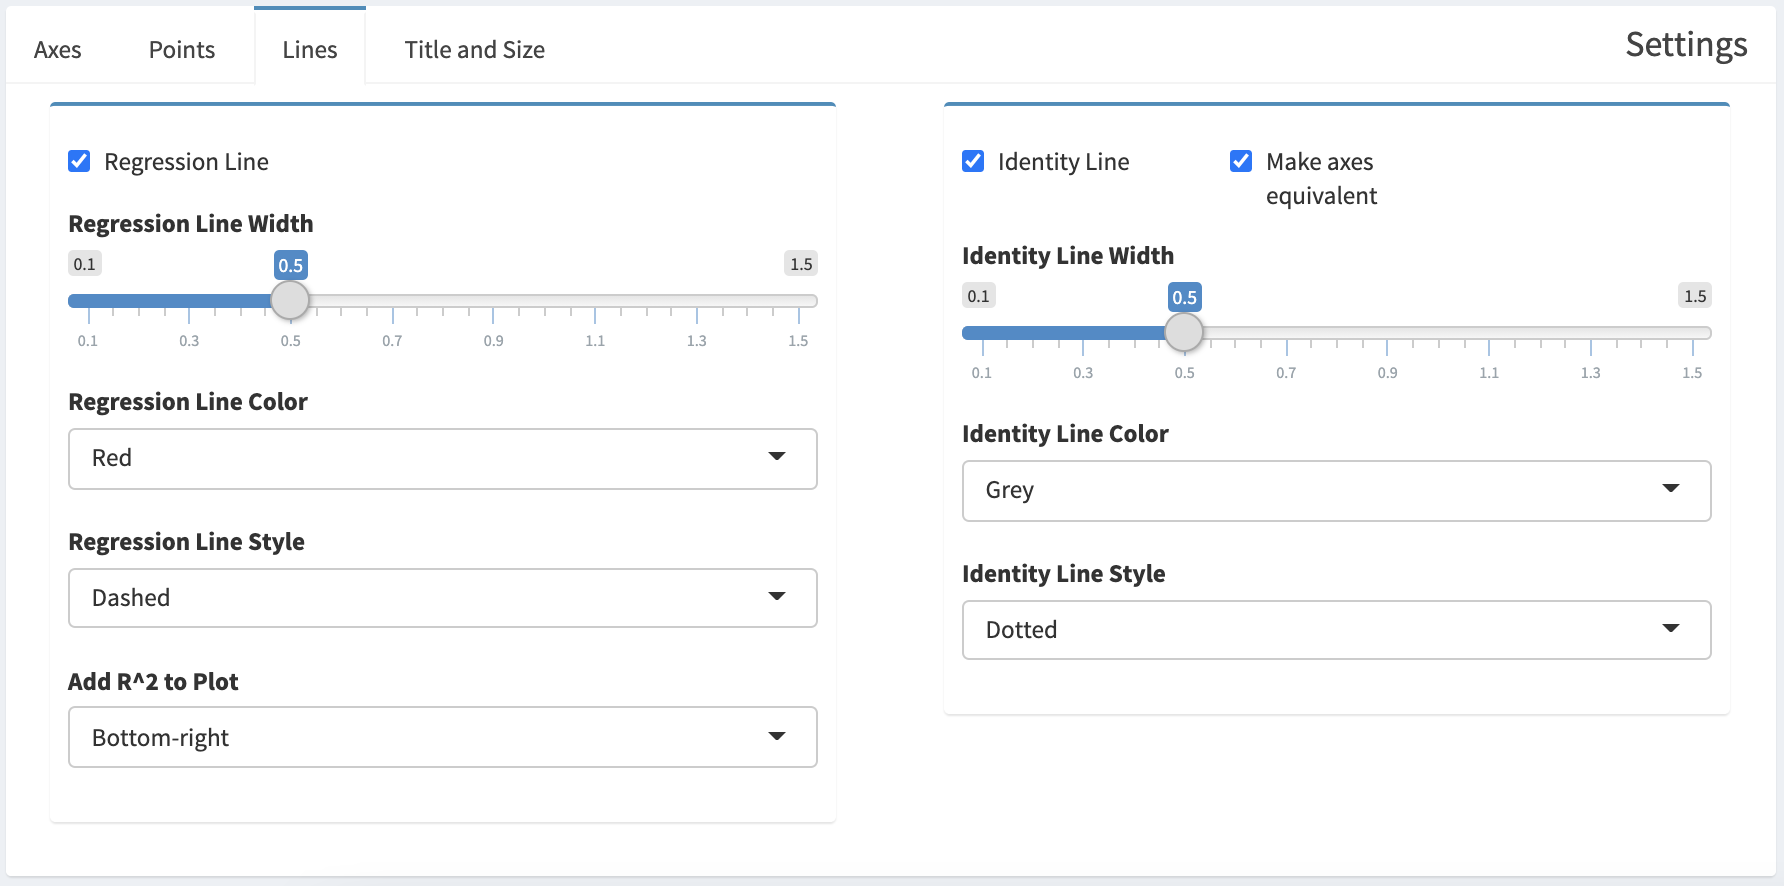
\includegraphics{images/Scatter_Lines.png}
\caption{The Lines tab in the Plot Settings box.}
\end{figure}

A linear regression line can be added to the plot by selecting \textbf{Regression Line}. The width of the line can be adjusted with the \textbf{Regression Line Width} slider, it can be colored by selecting a color from \textbf{Regression Line Color}, and the plotting style (solid, dashed, dotted, etc.) can be selected from the \textbf{Regression Liney Style} select box. An \(R^2\) of the correlation can be added to the plot by selecting an position option from the \textbf{Add R\^{}2 to Plot} select box.

An identity line can be added to the plot by selecting \textbf{Identity Line}. Identity lines are useful to illustrate the expected, perfect one-to-one relationship between two variables. Selecting \textbf{Make axes equivalent} will create a square plot in which the extents of the X- and Y-axes are the same. The identity line can be adjusted for width with the \textbf{Identity Line Width} slider, the color can be selected from the \textbf{Identity Line Color} select box, and the plotting style selected from the \textbf{Identity Line Style} select box.

\hypertarget{title-and-size-2}{%
\subsection{Title and Size}\label{title-and-size-2}}

\begin{figure}
\centering
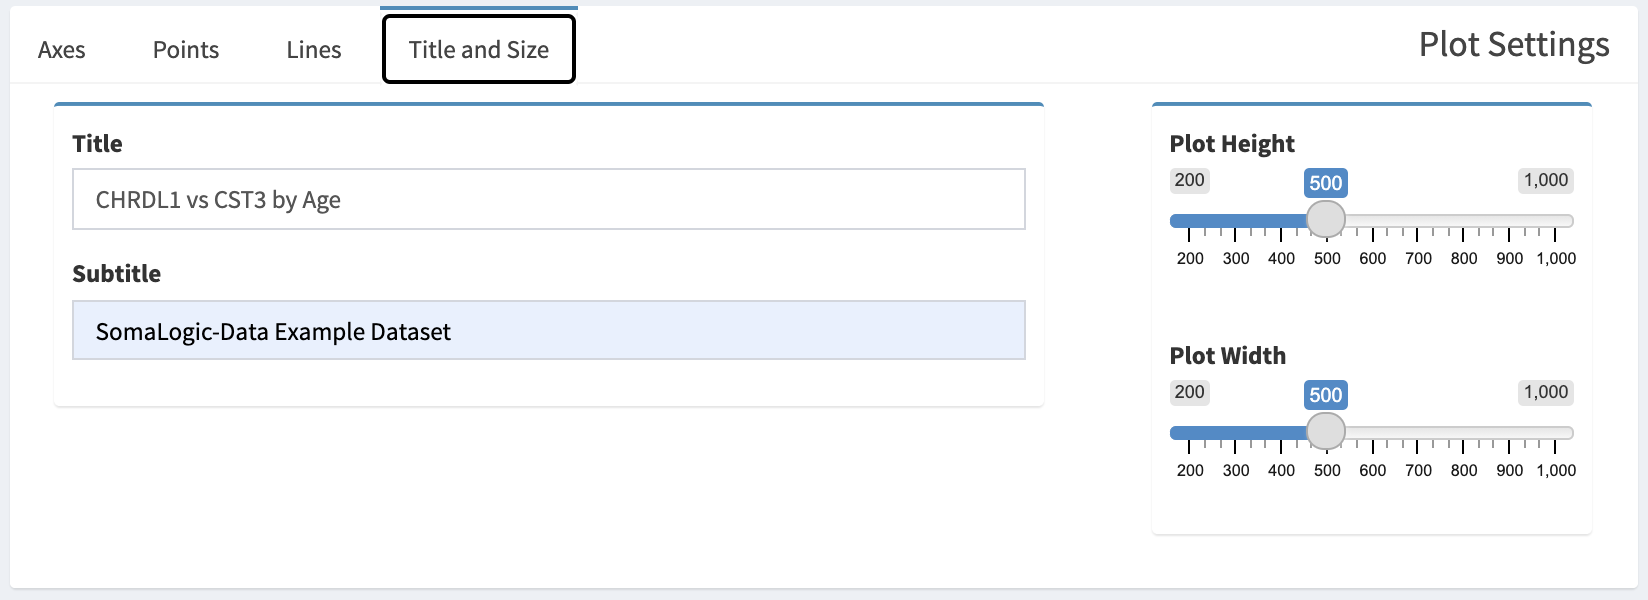
\includegraphics{images/Scatter_TitleSize.png}
\caption{The Title and Size tab int he Plot Settings box.}
\end{figure}

A title and subtitle can be added to the plot by entering text into the \textbf{Title} and \textbf{Subtitle} boxes. The plot size can be adjusted using the \textbf{Plot Height} and \textbf{Plot Width} sliders.

\hypertarget{statistical-tests}{%
\chapter{Statistical Tests}\label{statistical-tests}}

\begin{figure}
\centering
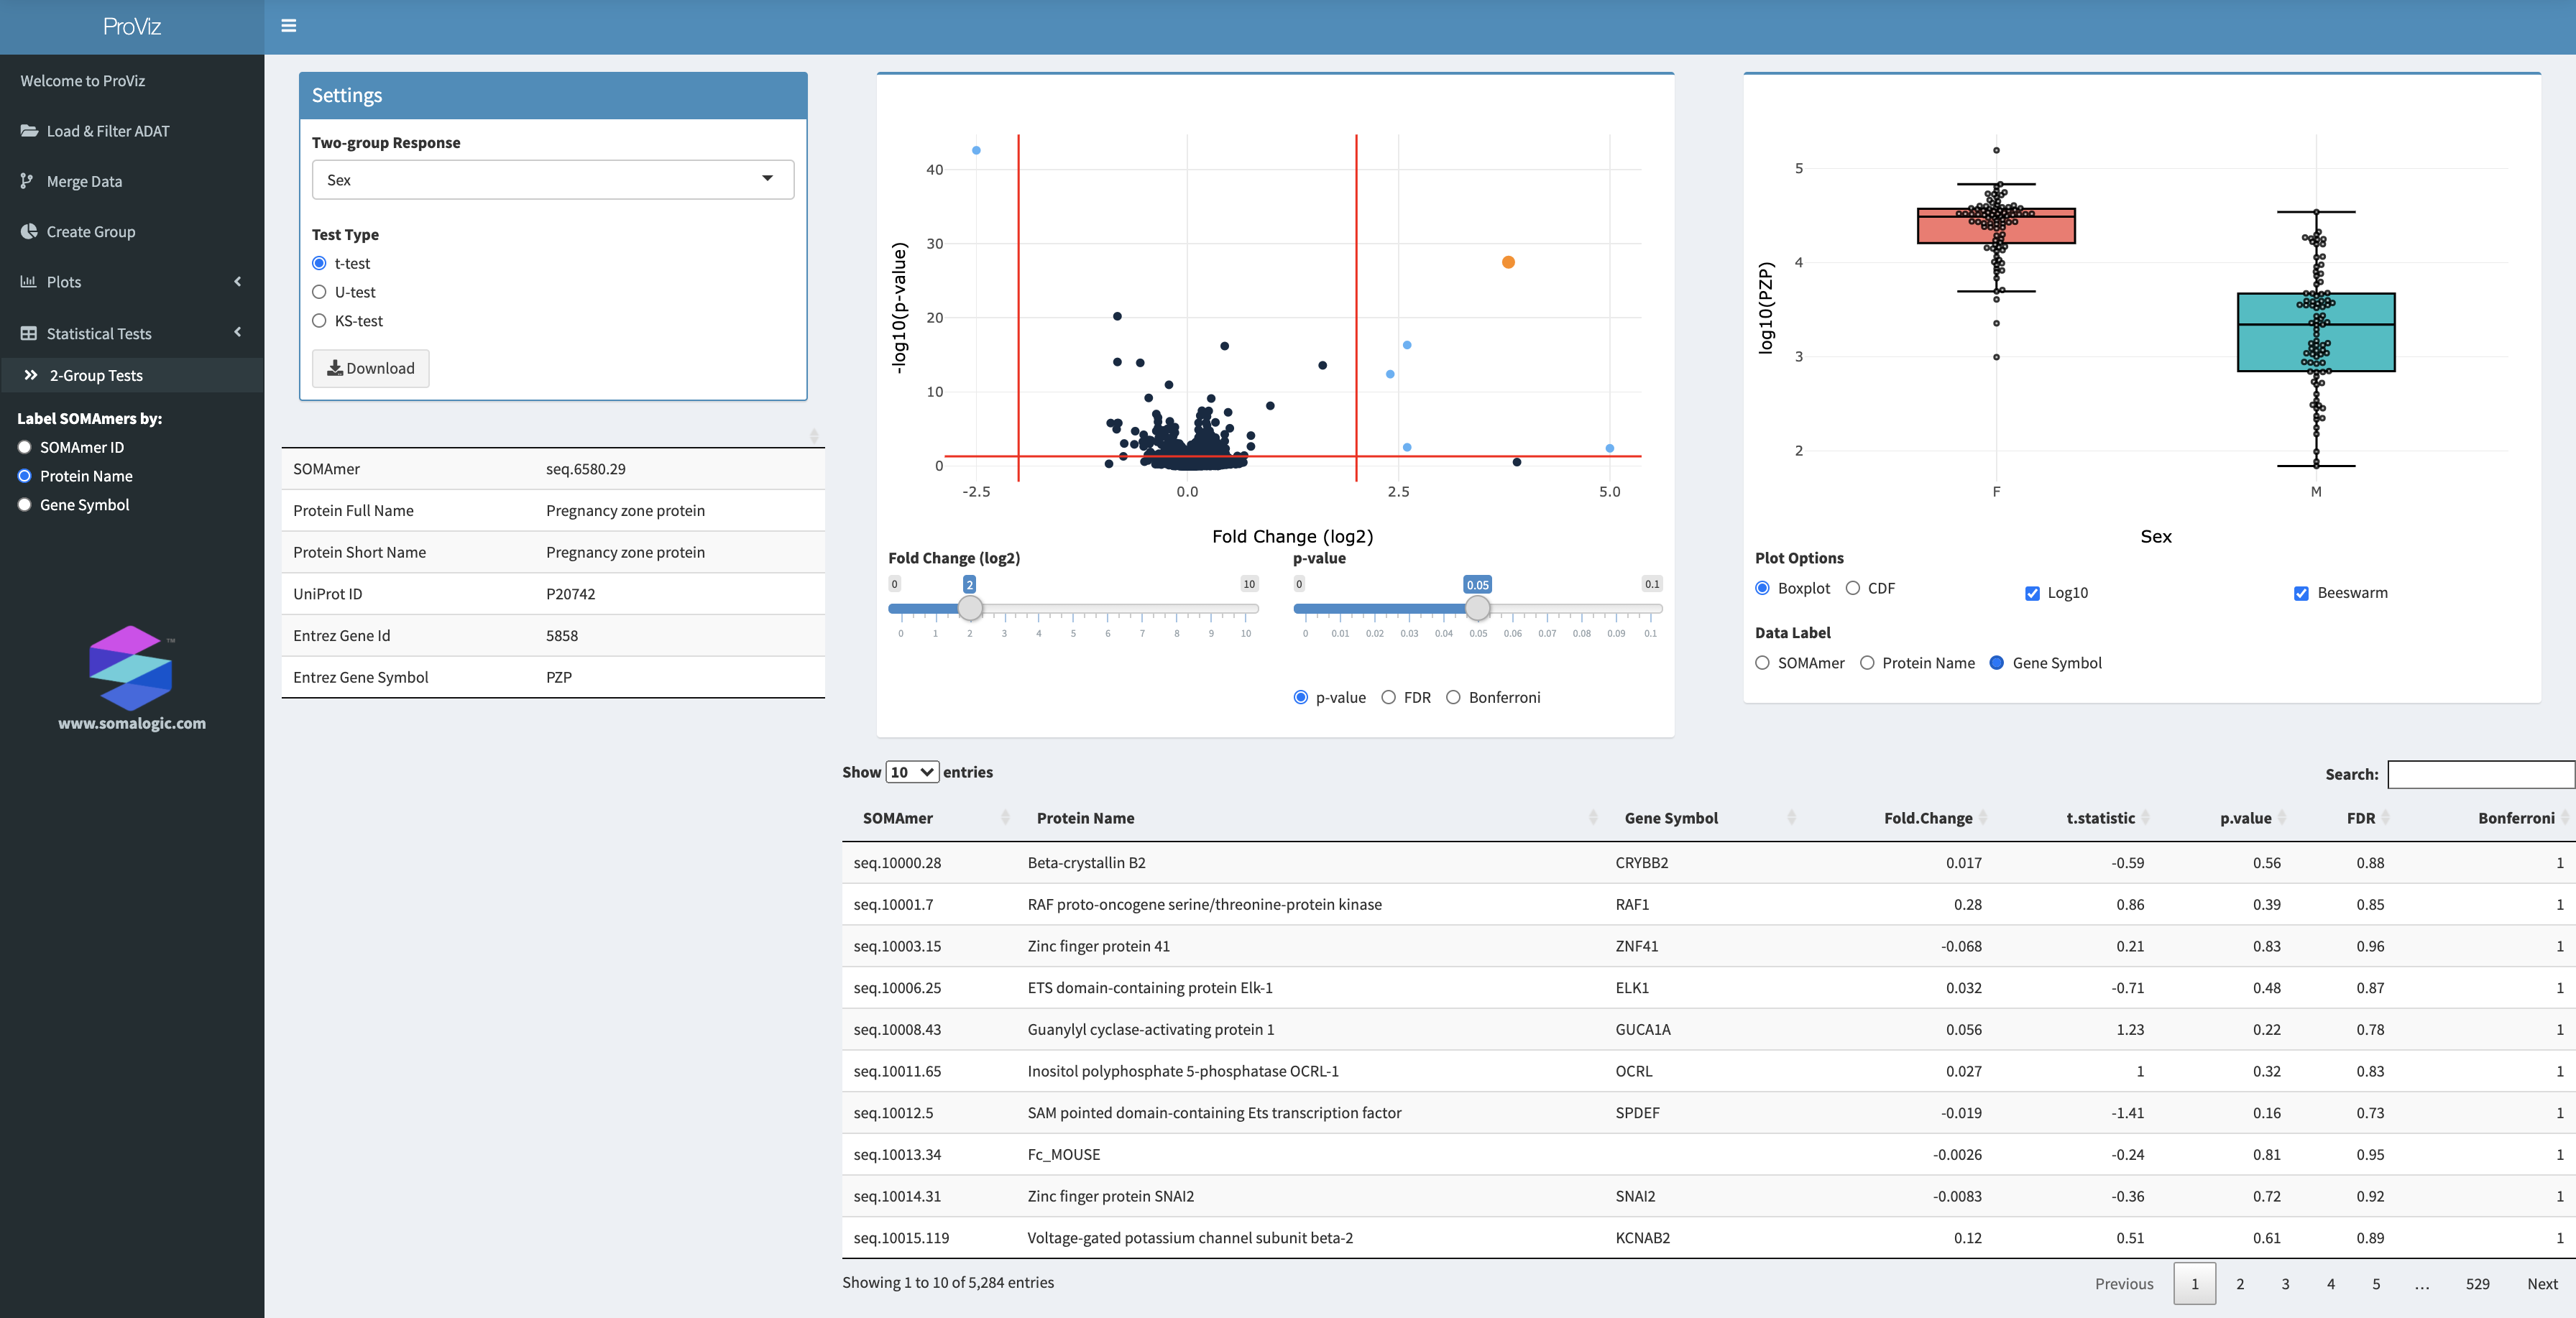
\includegraphics{images/StatTest_panel.png}
\caption{The Statistical Tests panel.}
\end{figure}

\hypertarget{statistical-tests-1}{%
\section{Statistical Tests}\label{statistical-tests-1}}

Different statistical tests for comparing continuous, two-group data, or multi-group data can be performed on the Statistical Tests panel. The tests available are:

\begin{itemize}
\item
  correlation - compares two continuous variables using either Pearson's or Spearman's rank-based methods
\item
  t-test - compares the means of two groups; a paired t-test is also available
\item
  U-test - compares the medians of two groups; this is a non-parametric alternative to the t-test; a paired U-test is also available
\item
  KS-test - compares the distributions of data between two groups
\item
  ANOVA - Analysis of Variance test of the means of multiple groups; repeated measures ANOVA is also available
\item
  Kruskal-Wallis - compares the medians of multiple groups; this is a non-parametric alternative to ANOVA
\item
  Friedman's Test - a non-parametric alternative to repeated measures ANOVA
\end{itemize}

\hypertarget{selecting-a-response}{%
\subsection{Selecting a Response}\label{selecting-a-response}}

\begin{figure}
\centering
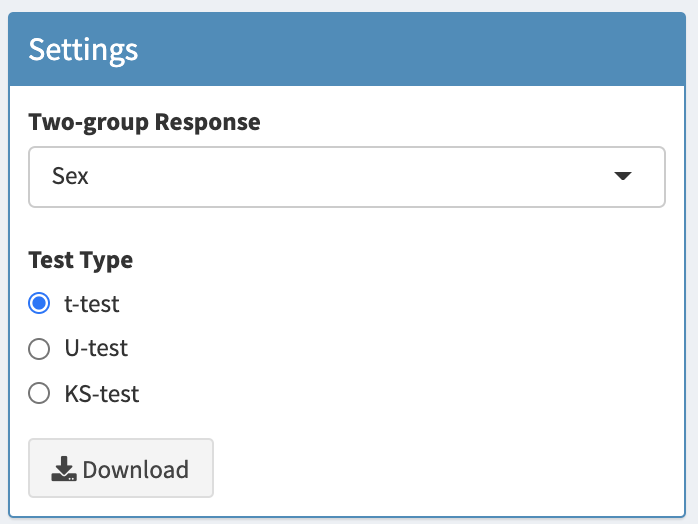
\includegraphics{images/StatTest_Settings.png}
\caption{The Settings box in the Statistical Tests panel.}
\end{figure}

The type of test can be selected from \textbf{Test Type}.

The variable containing the response or the grouping labels can be selected from the select box titled \textbf{Continuous Response}, \textbf{Two-group Response}, or \textbf{Multi-group Response}. The label of the select box will change as different test types are selected. Also, the contents of the select box will be updated with varaibles consistent with the selected test. After selecting a new response variable, tests will be performed for all SOMAmers in the ADAT, which could take a minute or two.

If a paired t-test, paired U-test, repeated measures ANOVA, or Friedman's test are required, check the Matched Samples box and select the variable which defines how samples are matched across groups. \textbf{All matched tests require a complete dataset in which each treatment group consists of the same number of matched subjects, and all subjects have measurements in each group. If your dataset is incomplete and does not have all measurements for all subjects across all groups, ProViz will attempt to adjust the data as necessary. This may, however result in errors.}

Once a test has been conducted, the \emph{Statistical Results Table} will contain all test results and can be downloaded as a comma-separated file (.csv) by clicking the \textbf{Download Results} button.

\hypertarget{plots-1}{%
\subsection{Plots}\label{plots-1}}

\begin{figure}
\centering
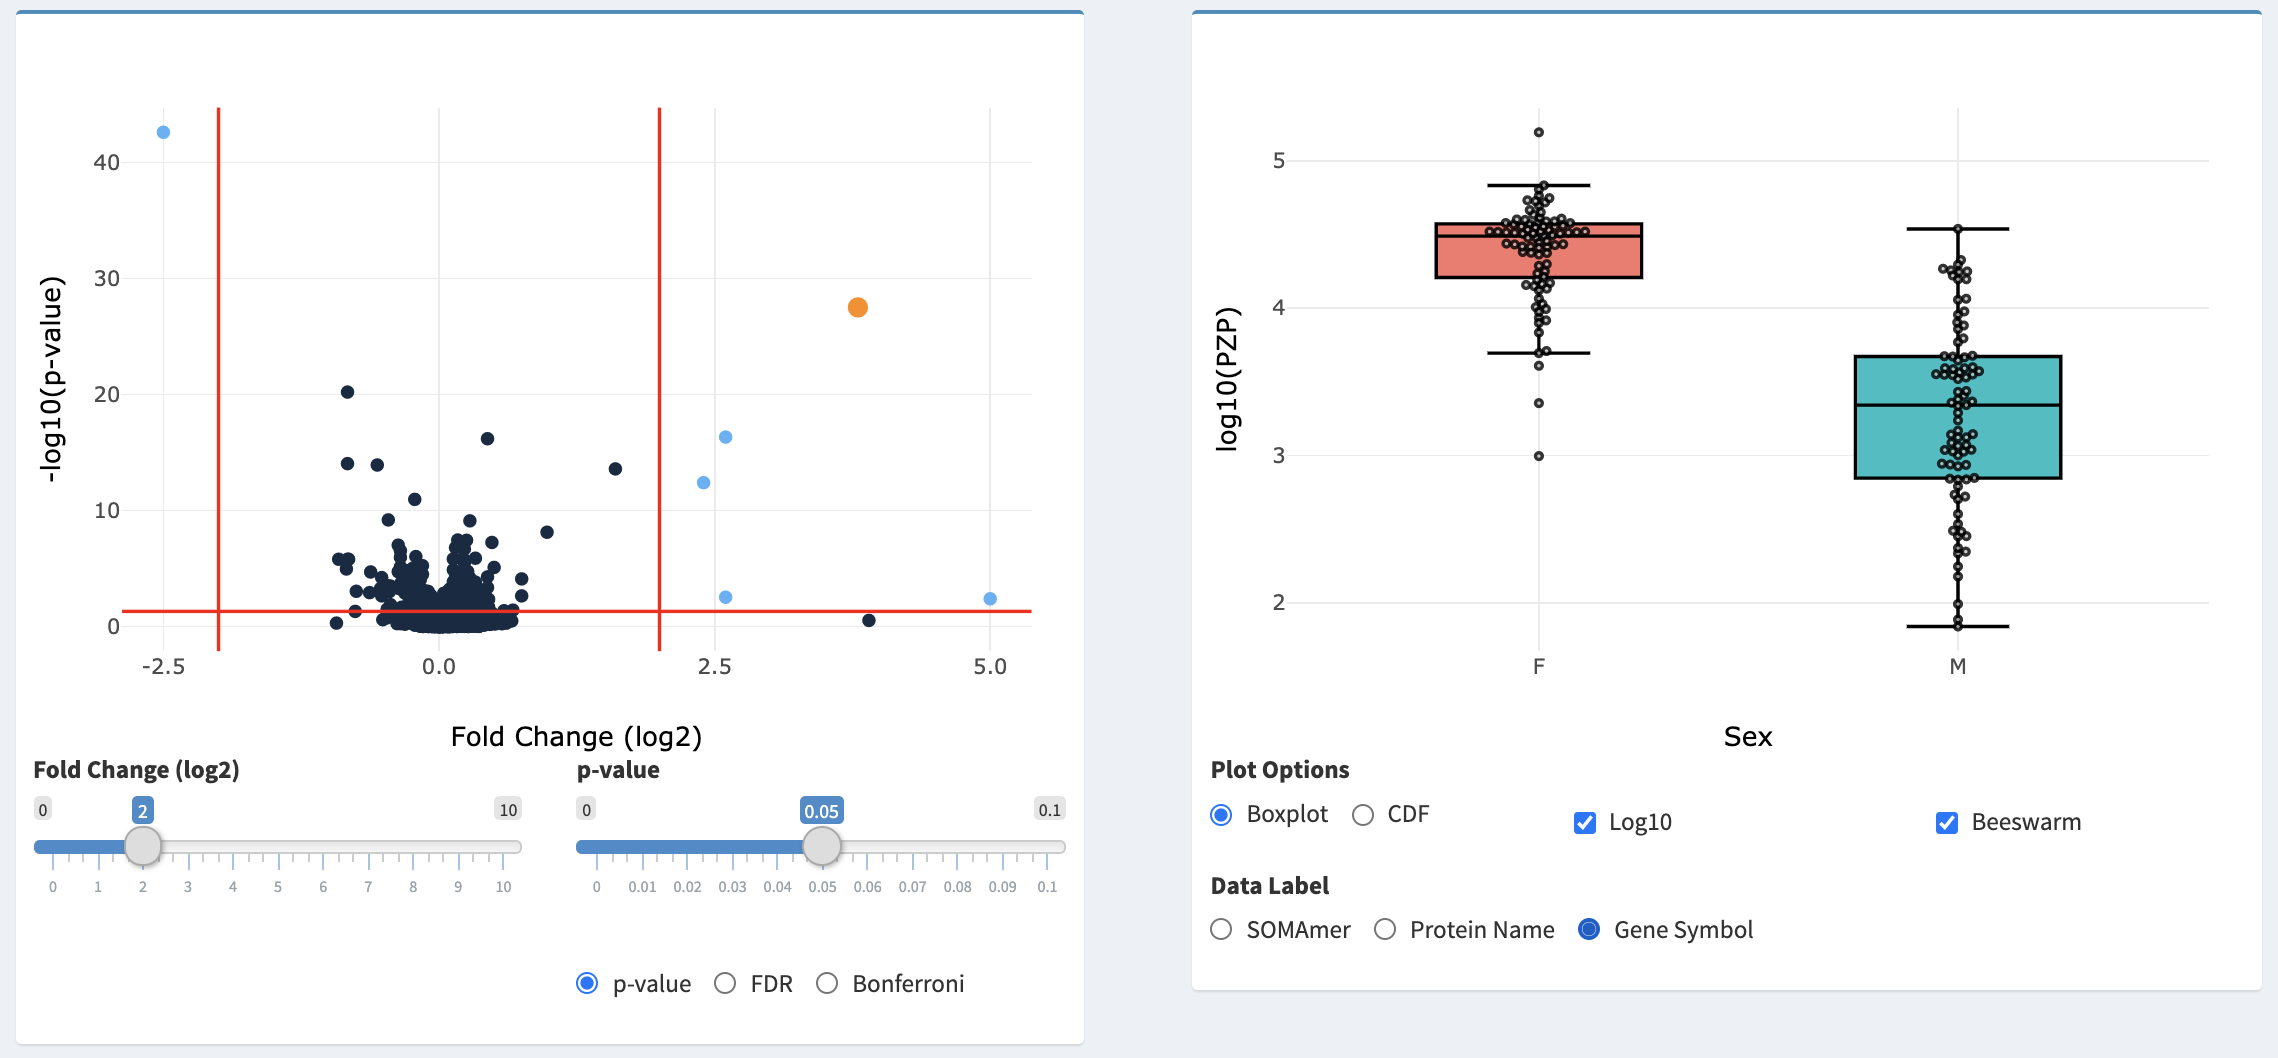
\includegraphics{images/StatTest_Volcano.png}
\caption{The Volcano Plot and Distribution Plot in the Statistical Tests panel.}
\end{figure}

After the statistical test is complete and the results table has been loaded, a volcano plot is displayed. For the t-test and U-test, this plot illustrates each SOMAmer as a point with the X-axis being the log2(fold change) and the Y-axis being -log10(p-value). For a correlation test, the X-axis will illustrate the Pearson's Correlation Coefficient. For ANOVA and Kruskal-Wallis, the X-axis will illustrate the maximum fold-change between groups. The left slider (\textbf{Fold Change (log2)} for all tests except correlation, and \textbf{Correlation} for the correlation test) and the \textbf{p-value} slider can be used to adjust the vertical and horizontal red lines in the plot, which represent cutoff values for identifying biomarkers of interest. Selecting \emph{p-value}, \emph{FDR}, or \emph{Bonferroni} will determine which type of p-value correction is used for plotting.

Hovering over points on the volcano plot will provide a pop-out detailing information of the SOMAmer associated with that point. Additionally, selecting a point by clicking on it will result in a plot illustrating the selected point's details. For correlation tests, a scatter plot of the SOMAmer data versus the response will be displayed. For all other tests, boxplots or CDF plots for that SOMAmer are shown - the plot can be changed between boxplot and CDF by selecting under \textbf{Plot Options}. Data can be log10 transformed by selecting \textbf{Log10} and individual points can be displayed by selecting \textbf{Beeswarm}. Hovering over points on this plot will provide additional information about the specific sample associated with that point, and hovering over the boxplot will provide summary statistics. The Y-axis of the plot can be labeled with the SOMAmer Id, Protein Name, or Gene Symbol by selecting the appropriate item under \textbf{Data Label}.

For matched tests, matched observations across groups can be connected with lines by selecting the \textbf{Plot Matched} checkbox on the Distribution Plot.

\hypertarget{statistical-results-table}{%
\subsection{Statistical Results Table}\label{statistical-results-table}}

\begin{figure}
\centering
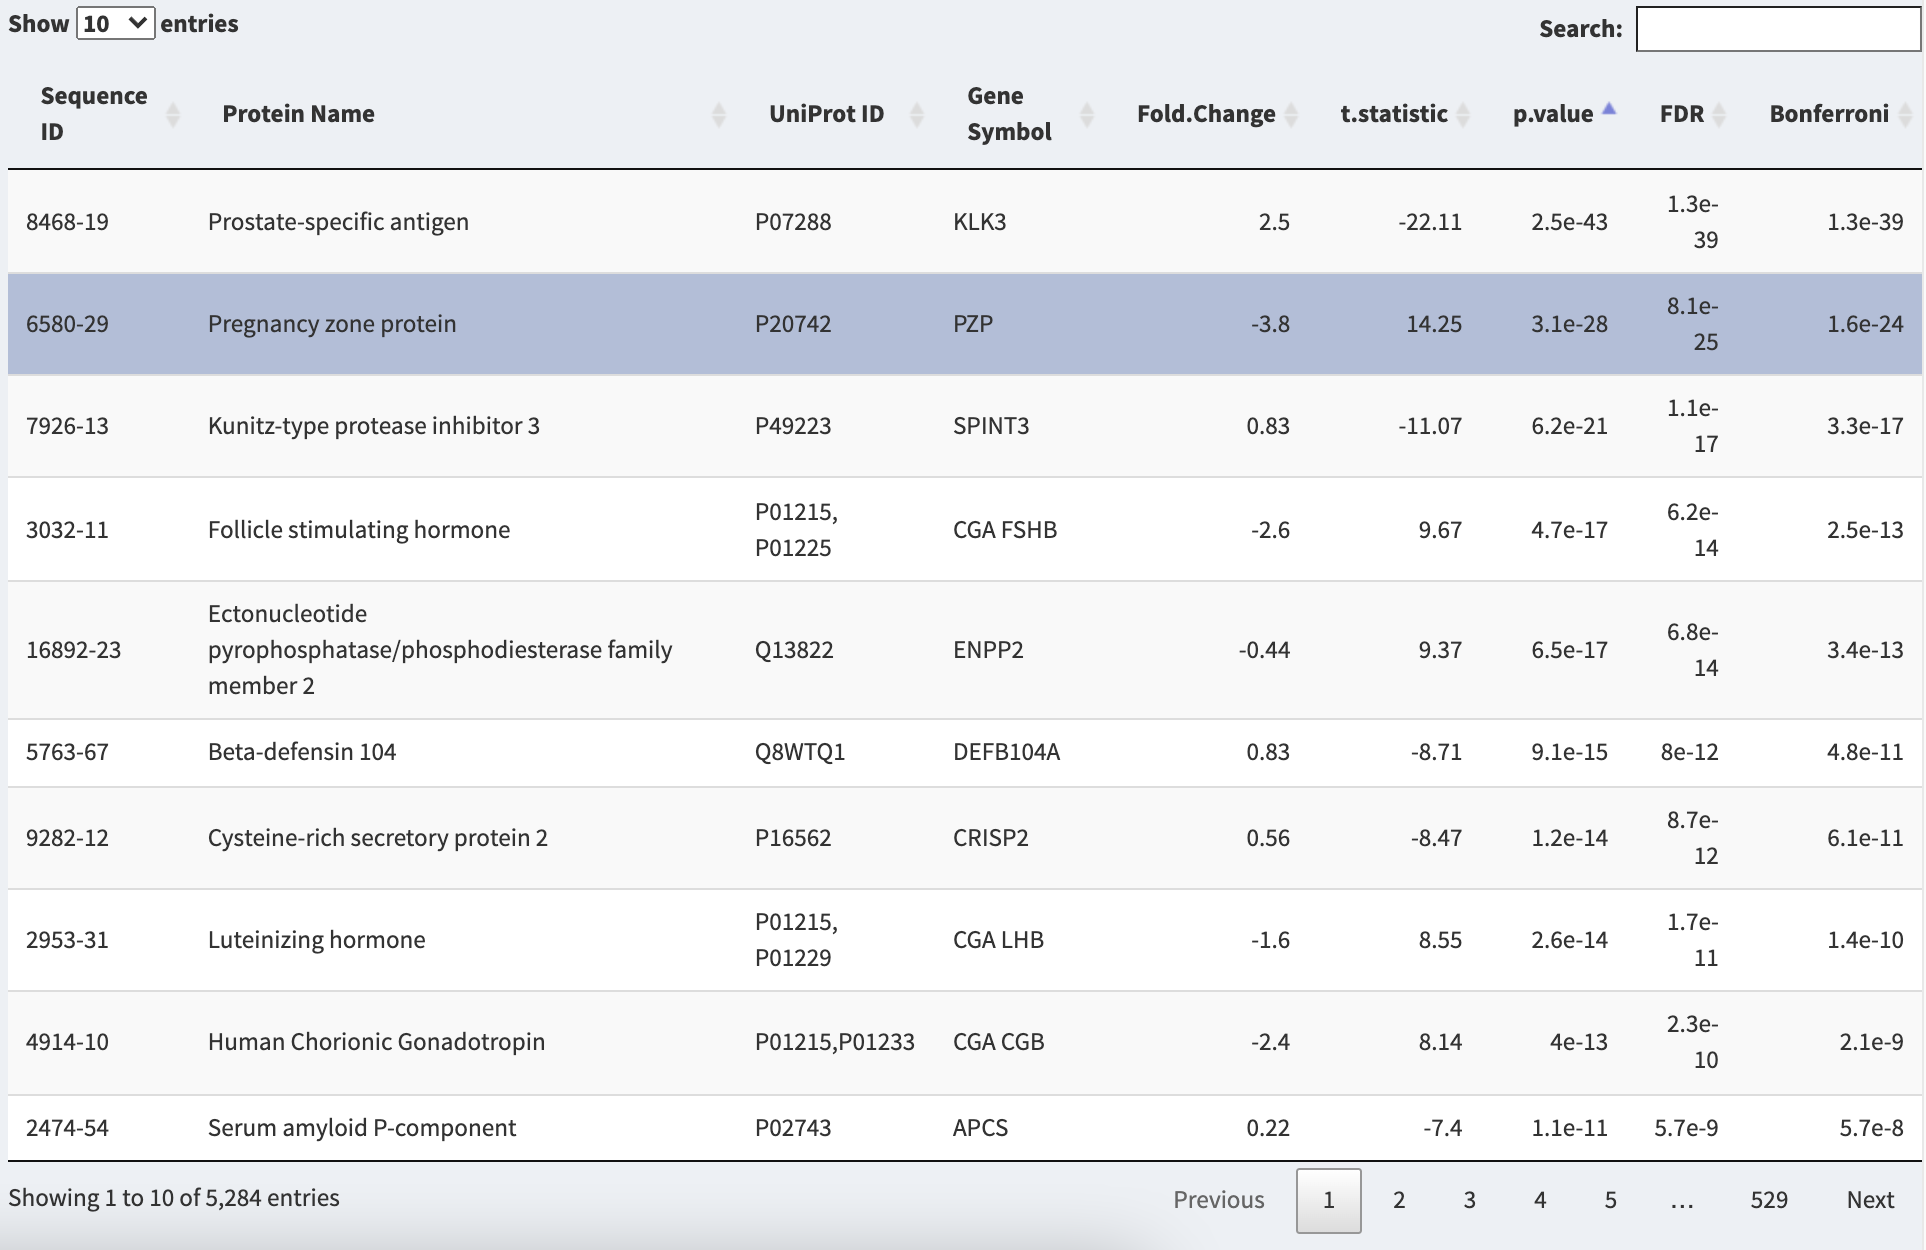
\includegraphics{images/StatTest_ResultsTable.png}
\caption{The Statistical Results Table in the Statistical Tests panel.}
\end{figure}

Results of the statistical test performed for all SOMAmers will be displayed in the \textbf{Statistical Results Table}. All protein identifiers (\emph{SOMAmer Id}, \emph{Protein Name}, \emph{Gene Symbol}) will be displayed along with \emph{Fold Change}, \emph{Maximum Fold Change}, or \emph{r} (Pearson's correlation coefficient), depending on the chosen test. Additional columns contain, the test statistic, p-value, and p-values adjusted for multiple testing by False Discovery Rate (FDR) or Bonferroni correction. The table can be sorted by clicking on the double arrow next to any column name, or searched for protein name or gene symbol. Selecting a row in the table will result in that point being illustrated in the volcano plot as well as a distribution or scatter plot.

\end{document}
